\documentclass{article}

\usepackage{array,calc} 
\usepackage{graphics}
\usepackage{amsmath}
%\usepackage{indentfirst}
\usepackage[utf8]{inputenc}
\usepackage{url}
\usepackage{fullpage}

\newcommand{\blam}{ \mbox{\boldmath $ \lambda $} }
\newcommand{\bet}{ \mbox{\boldmath $ \eta $} }
\newcommand{\bome}{ \mbox{\boldmath $ \omega $} }
\newcommand{\bbet}{ \mbox{\boldmath $ \beta $} }
\newcommand{\bbeta}{ \mbox{\boldmath $ \beta $} }
\newcommand{\balph}{ \mbox{\boldmath $ \alpha $} }
\newcommand{\balpha}{ \mbox{\boldmath $ \alpha $} }
\newcommand{\bphi}{ \mbox{\boldmath $\phi$}}
\newcommand{\bzeta}{ \mbox{\boldmath $\zeta$}}
\newcommand{\bkap}{ \mbox{\boldmath $\kappa$}}
\newcommand{\bkappa}{ \mbox{\boldmath $\kappa$}}
\newcommand{\beps}{ \mbox{\boldmath $\epsilon$}}
\newcommand{\bepsilon}{ \mbox{\boldmath $\epsilon$}}
\newcommand{\bthet}{ \mbox{\boldmath $ \theta $} }
\newcommand{\btheta}{ \mbox{\boldmath $ \theta $} }
\newcommand{\bnu}{ \mbox{\boldmath $\nu$} }
\newcommand{\bmu}{ \mbox{\boldmath $\mu$} }
\newcommand{\bGam}{ \mbox{\boldmath $\Gamma$} }
\newcommand{\bSig}{ \mbox{\boldmath $\Sigma$} }
\newcommand{\bSigma}{ \mbox{\boldmath $\Sigma$} }
\newcommand{\bPhi}{ \mbox{\boldmath $\Phi$} }
\newcommand{\bThet}{ \mbox{\boldmath $\Theta$} }
\newcommand{\bTheta}{ \mbox{\boldmath $\Theta$} }
\newcommand{\bDel}{ \mbox{\boldmath $\Delta$} }
\newcommand{\bDelta}{ \mbox{\boldmath $\Delta$} }
\newcommand{\bnabla}{ \mbox{\boldmath $\nabla$} }
\newcommand{\bLam}{ \mbox{\boldmath $\Lambda$} }
\newcommand{\bLambda}{ \mbox{\boldmath $\Lambda$} }
\newcommand{\bgam}{ \mbox{\boldmath $\gamma$} }
\newcommand{\bgamma}{ \mbox{\boldmath $\gamma$} }
\newcommand{\brho}{ \mbox{\boldmath $\rho$} }
\newcommand{\bdel}{ \mbox{\boldmath $\delta$} }
\newcommand{\bdelta}{ \mbox{\boldmath $\delta$} }

\newcommand{\sis}{\sigma^2}

\newcommand{\bzero}{\textbf{0}}
\newcommand{\bones}{\textbf{1}}
\newcommand{\ba}{\textbf{a}}
\newcommand{\bs}{\textbf{s}}
\newcommand{\bt}{\textbf{t}}
\newcommand{\bu}{\textbf{u}}
\newcommand{\bv}{\textbf{v}}
\newcommand{\bw}{\textbf{w}}
\newcommand{\bW}{\textbf{W}}
\newcommand{\bx}{\textbf{x}}
\newcommand{\bX}{\textbf{X}}
\newcommand{\by}{\textbf{y}}
\newcommand{\bY}{\textbf{Y}}
\newcommand{\bz}{\textbf{z}}
\newcommand{\bZ}{\textbf{Z}}


\newcommand{\matern}{\mbox{Mat\'{e}rn }}
\newcommand{\mbf}[1]{\mbox{\boldmath$#1$}}
\newcommand{\Cov}{\mbox{Cov}}
\newcommand{\Diag}{\mbox{Diag}}

\newcommand{\bc}{\begin{center}}
\newcommand{\ec}{\end{center}}
\newcommand{\beq}{\begin{equation}}
\newcommand{\eeq}{\end{equation}}
\newcommand{\bea}{\begin{eqnarray}}
\newcommand{\eea}{\end{eqnarray}}
\newcommand{\beas}{\begin{eqnarray*}}
\newcommand{\eeas}{\end{eqnarray*}}
\newcommand{\bi}{\begin{itemize}}
\newcommand{\ei}{\end{itemize}}
\newcommand{\bis}{\begin{itemstep}}
\newcommand{\eis}{\end{itemstep}}
\newcommand{\bqu}{\begin{quote}}
\newcommand{\equ}{\end{quote}}
\newcommand{\bdes}{\begin{description}}
\newcommand{\edes}{\end{description}}
\newcommand{\be}{\begin{enumerate}}
\newcommand{\ee}{\end{enumerate}}
\newcommand{\nn}{\nonumber}
\newcommand{\bex}{\begin{example} \rm }
\newcommand{\eex}{\rule{5pt}{5pt} \end{example}}
\newcommand{\bdf}{\begin{definition} \rm }
\newcommand{\edf}{\end{definition}}
\newcommand{\bthm}{\begin{theorem} \rm }
\newcommand{\ethm}{\end{theorem}}
\newcommand{\balg}{\begin{algorithm} \rm }
\newcommand{\ealg}{\end{algorithm}}
\newcommand{\np}{\newpage}

\newcommand{\mywid}{2.1in}
\newcommand{\mywidr}{2.2in}
\newcommand{\myht}{1.5in}
\newcommand{\myhts}{1.1in}
\newcommand{\myupvspace}{-\myht}
\newcommand{\myupvspaces}{-\myhts}
\newcommand{\mydnvspace}{.3in}
\newcommand{\myhspace}{2.2in}
\newcommand{\myhmidspace}{1.1in}
\newcommand{\mybotvspace}{.1in}
\newcommand{\vsp}{\vspace{2ex}}

\newcommand{\proglang}[1]{{\textsf{#1}}}
\newcommand{\R}{\proglang{R}}
\newcommand{\pkg}[1]{{\normalfont\fontseries{b}\selectfont #1}}
\newcommand{\pbs}[1]{\let\tmp\\#1\let\\\tmp} 


 


\usepackage{Sweave}
\begin{document}


\title{Hierarchical Modeling for Univariate Spatial Data in \proglang{R}: LiDAR and Forest Biomass Example}

\author{Andrew O. Finley and Sudipto Banerjee}
\maketitle

\section{Data preparation and initial exploration}

We make use of several libraries in the following example session, including:

\begin{tabular}{*2{>{\pbs{\raggedright}}p{\columnwidth/2 -3\tabcolsep}}}
  \begin{itemize}\setlength{\itemsep}{-0.05cm}
  \item \verb@library(fields)@
  \item \verb@library(geoR)@
  \item \verb@library(MBA)@
  \item \verb@library(raster)@
  \end{itemize}
  &
  \begin{itemize}\setlength{\itemsep}{-0.05cm}
  \item \verb@library(rgdal)@
  \item \verb@library(RgoogleMaps)@
  \item \verb@library(spBayes)@
  \item \verb@library(yaImpute)@
  \end{itemize}
\end{tabular} 


The study area is the US Forest Service Penobscot Experimental Forest (PEF; \url{www.fs.fed.us/ne/durham/4155/penobsco.htm}), ME, USA. The dataset comprises LiDAR waveforms collected with the Laser Vegetation Imaging Sensor (LVIS; \url{http://lvis.gsfc.nasa.gov}) and several forest variables measured on a set of 589 georeferenced forest inventory plots. The LVIS data were acquired during the summer of 2003. The LVIS instrument, an airborne scanning LiDAR with a 1064 nm laser, provided 12414 LiDAR waveform signals within the PEF. For each waveform, elevations were converted to height above the ground surface and interpolated at 0.3 m intervals. 

We use these data to demonstrate some basics of spatial data manipulation, visualization, and univariate spatial regression analysis. The regression models can be used to make biomass prediction at a high spatial resolution across the PEF.

We begin by reading in the data, removing non-forest inventory plots, transforming biomass measurements to the square-root of metric tons per hectare, and taking a look at plot locations across the forest.

\section{Forest inventory data}
\begin{Schunk}
\begin{Sinput}
> PEF.shp <- readOGR("PEF-data", "PEF-bounds")
\end{Sinput}
\begin{Soutput}
OGR data source with driver: ESRI Shapefile 
Source: "PEF-data", layer: "PEF-bounds"
with 1 features and 5 fields
Feature type: wkbPolygon with 2 dimensions
\end{Soutput}
\begin{Sinput}
> PEF.poly <- as.matrix(PEF.shp@polygons[[1]]@Polygons[[1]]@coords)
> PEF.plots <- read.csv("PEF-data/PEF-plots.csv")
> PEF.plots <- PEF.plots[sapply(PEF.plots[, "biomass.mg.ha"], function(x) {
+     !any(is.na(x))
+ }), ]
> coords <- PEF.plots[, c("easting", "northing")]
> bio <- sqrt(PEF.plots$biomass.mg.ha)
> plot(coords, pch = 19, cex = 0.5, xlab = "Easting (m)", ylab = "Northing (m)")
> plot(PEF.shp, add = TRUE, usePolypath = FALSE)
\end{Sinput}
\end{Schunk}

\begin{figure}
\begin{center}
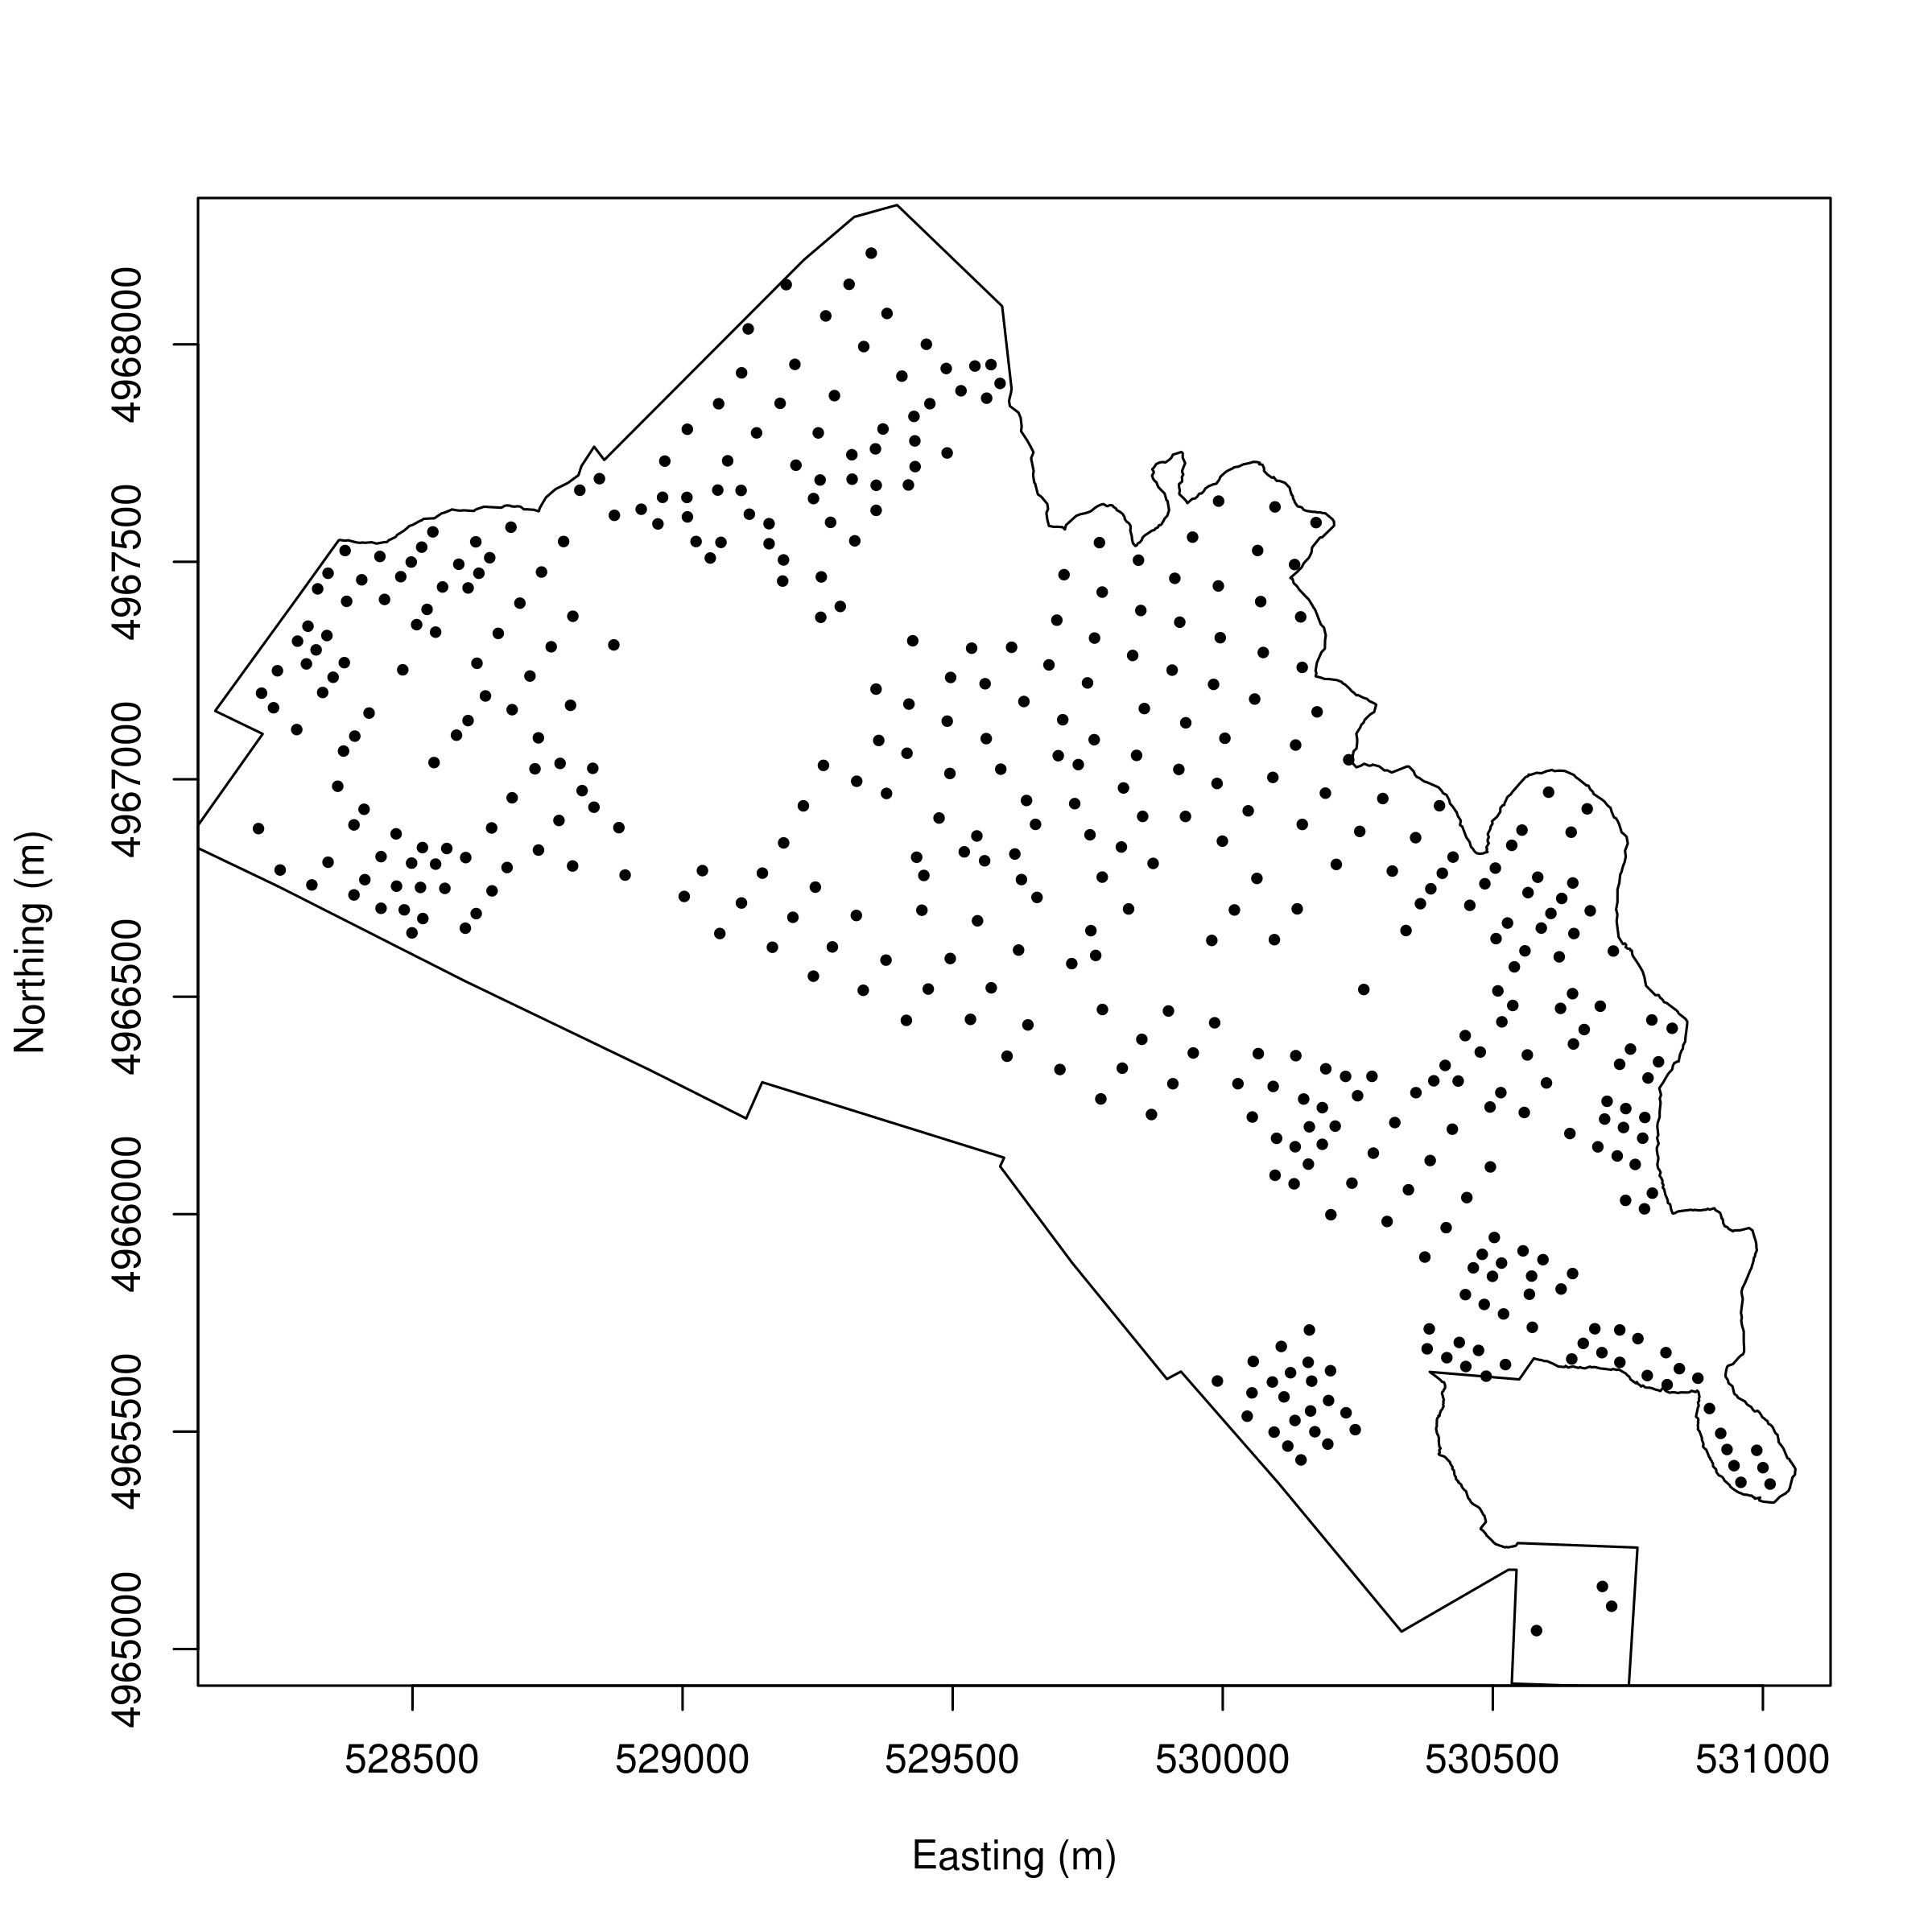
\includegraphics[width=10cm]{figures/fig-coords}
\end{center}
\caption{Forest inventory plot locations across the PEF.}
\label{fig:fig-coords}
\end{figure}

Our objective is to obtain an estimate, with an associated measure of uncertainty, of biomass as a continuous surface over the domain. We can gain a non-statistical estimate of this surface using the \pkg{MBA} package which provides efficient interpolation of large data sets using multilevel B-splines. The result of the \verb@mba.surf@ function can be passed to \verb@image@ or \verb@image.plot@ to produce $\Re^2$ depictions, Figure~\ref{fig:MBASurf}.

\begin{Schunk}
\begin{Sinput}
> surf <- mba.surf(cbind(coords, bio), no.X = 200, no.Y = 200, extend = FALSE)$xyz.est
> image.plot(surf, xaxs = "r", yaxs = "r", xlab = "Easting (m)", ylab = "Northing (m)")
> plot(PEF.shp, add = TRUE, usePolypath = FALSE)
> points(coords)
\end{Sinput}
\end{Schunk}

\begin{figure}
\begin{center}
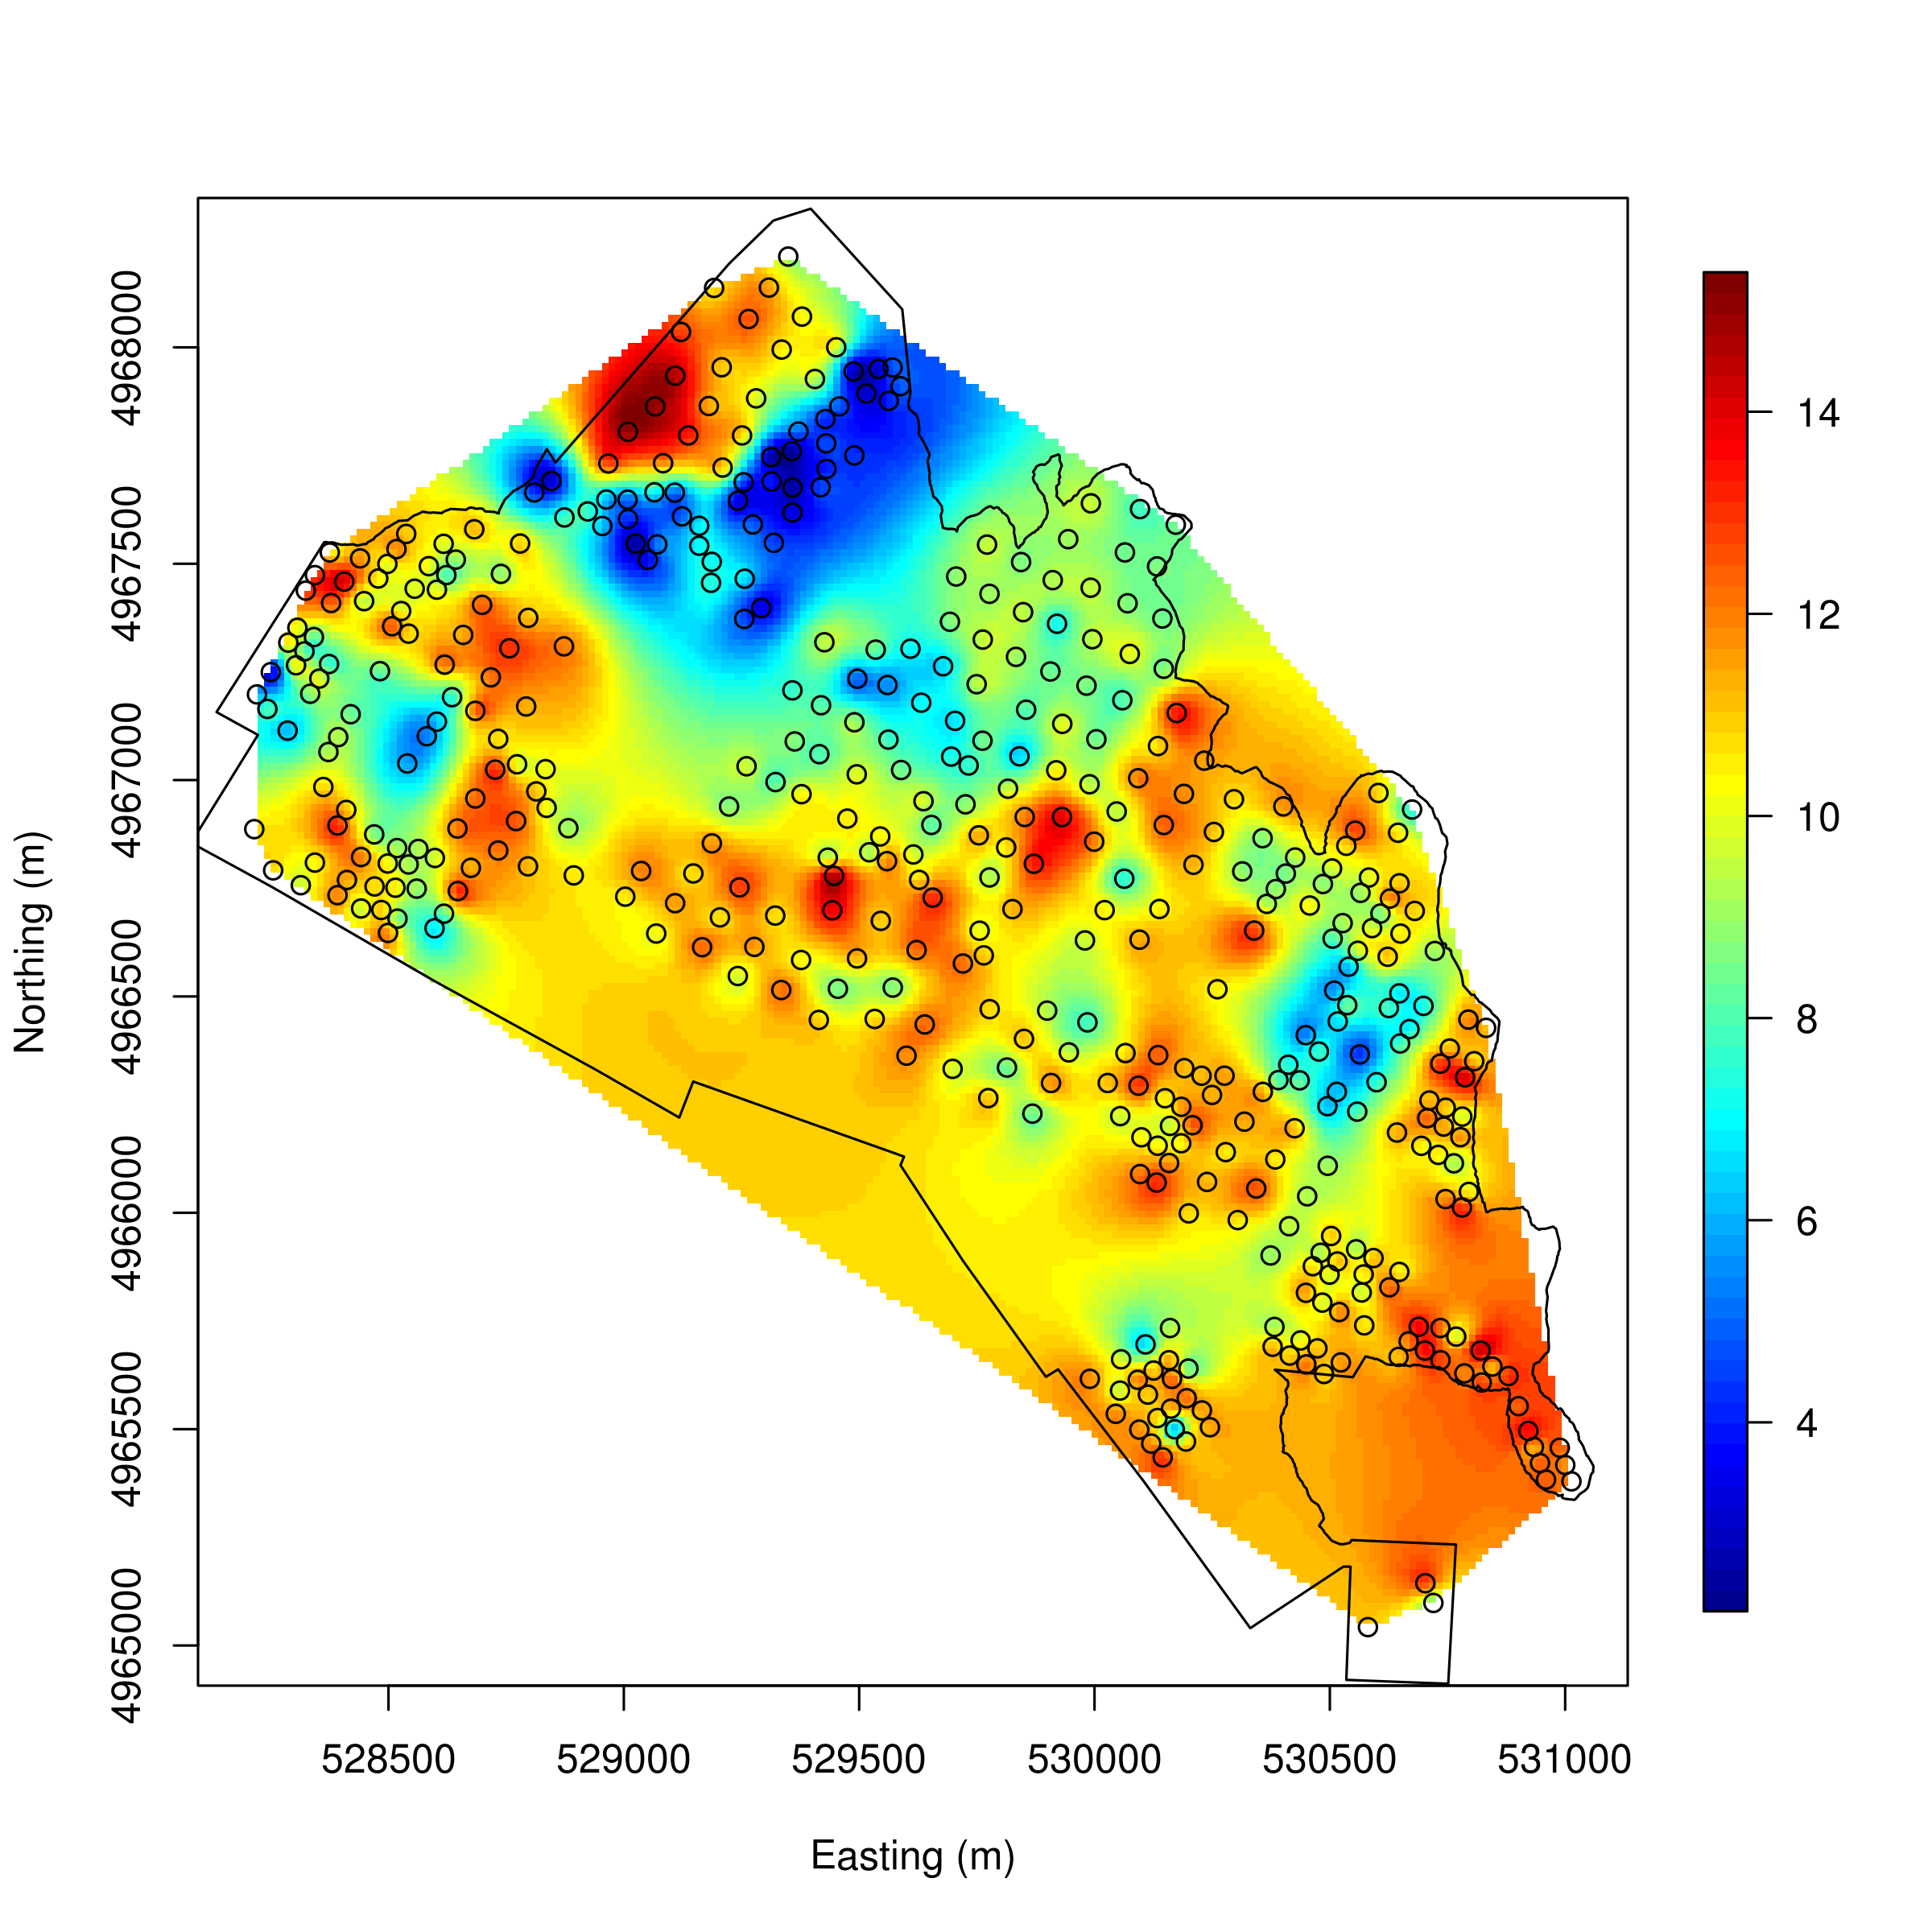
\includegraphics[width=10cm]{figures/fig-MBASurf}
\end{center}
\caption{Interpolation of square-root metric tons of biomass using a Multilevel B-spline.}
\label{fig:MBASurf}
\end{figure}

\section{LiDAR derived covariates}
We hope to improve prediction by using information in the LiDAR signals. First, however, we need a way to extract useful covariates from these high-dimensional signals. Given we're working within a regression setting, these covariates cannot be highly correlated with each other, i.e., we need to avoid issues with \emph{multicollinearity}. One approach is to use Singular Value Decomposition (SVD) to extract those orthogonal vectors that explain some desired level of variance in LiDAR signals. 

In the code below, we read in the LiDAR data and define several functions that use the \verb@SVD@ function to extract singular vectors of the LiDAR data matrix. Here too, we provide some diagnostic plots useful for selecting the number of singular vectors to retain for use in the subsequent regression analysis.

\begin{Schunk}
\begin{Sinput}
> eof.fit <- function(X, p) {
+     s <- svd(X)
+     s$u[, 1:p] %*% diag(s$d[1:p]) %*% t(s$v[, 1:p])
+ }
> eof <- function(X, p) {
+     svd(X)$u[, 1:p]
+ }
> eof.summary <- function(X, per = c(25, 50, 95), col = c(1:3)) {
+     s <- svd(X)
+     svd.var <- s$d^2/sum(s$d^2) * 100
+     svd.cum.var <- cumsum(s$d^2/sum(s$d^2)) * 100
+     svd.per <- (1:ncol(X))[sapply(per, function(p) {
+         min(which(svd.cum.var >= p))
+     })]
+     svd.col <- cumsum(s$d[col]^2/sum(s$d^2)) * 100
+     list(var = svd.var, cum.var = svd.cum.var, per.exp = svd.per, 
+         per = per, col.exp = svd.col, col = col)
+ }
> lvis <- as.matrix(read.csv("PEF-data/PEF-LVIS.csv"))
> X <- scale(lvis[, 3:ncol(lvis)], scale = FALSE)
> eof.var <- eof.summary(X, per = c(50, 90, 95, 99), col = c(1:5))
> par(mfrow = c(1, 2), mar = c(4, 6, 4, 2))
> plot(eof.var[[1]], ylim = c(0, 100), cex.lab = 2, xlab = "SVD column", 
+     ylab = "Percent variance explained", pch = 19, cex = 0.2)
> abline(v = eof.var[[3]], col = rainbow(length(eof.var[[3]])))
> legend("topright", lty = 1, legend = paste("Column ", eof.var[[3]], 
+     ": ", eof.var[[4]], "%", sep = ""), col = rainbow(length(eof.var[[3]])), 
+     bty = "n")
> plot(eof.var[[2]], ylim = c(0, 100), cex.lab = 2, xlab = "SVD column", 
+     ylab = "Cumulative percent variance explained", pch = 19, cex = 0.2)
> abline(v = eof.var[[3]], col = rainbow(length(eof.var[[3]])))
> legend("bottomright", lty = 1, legend = paste("Column ", eof.var[[3]], 
+     ": ", eof.var[[4]], "%", sep = ""), col = rainbow(length(eof.var[[3]])), 
+     bty = "n")
\end{Sinput}
\end{Schunk}

\begin{figure}
\begin{center}
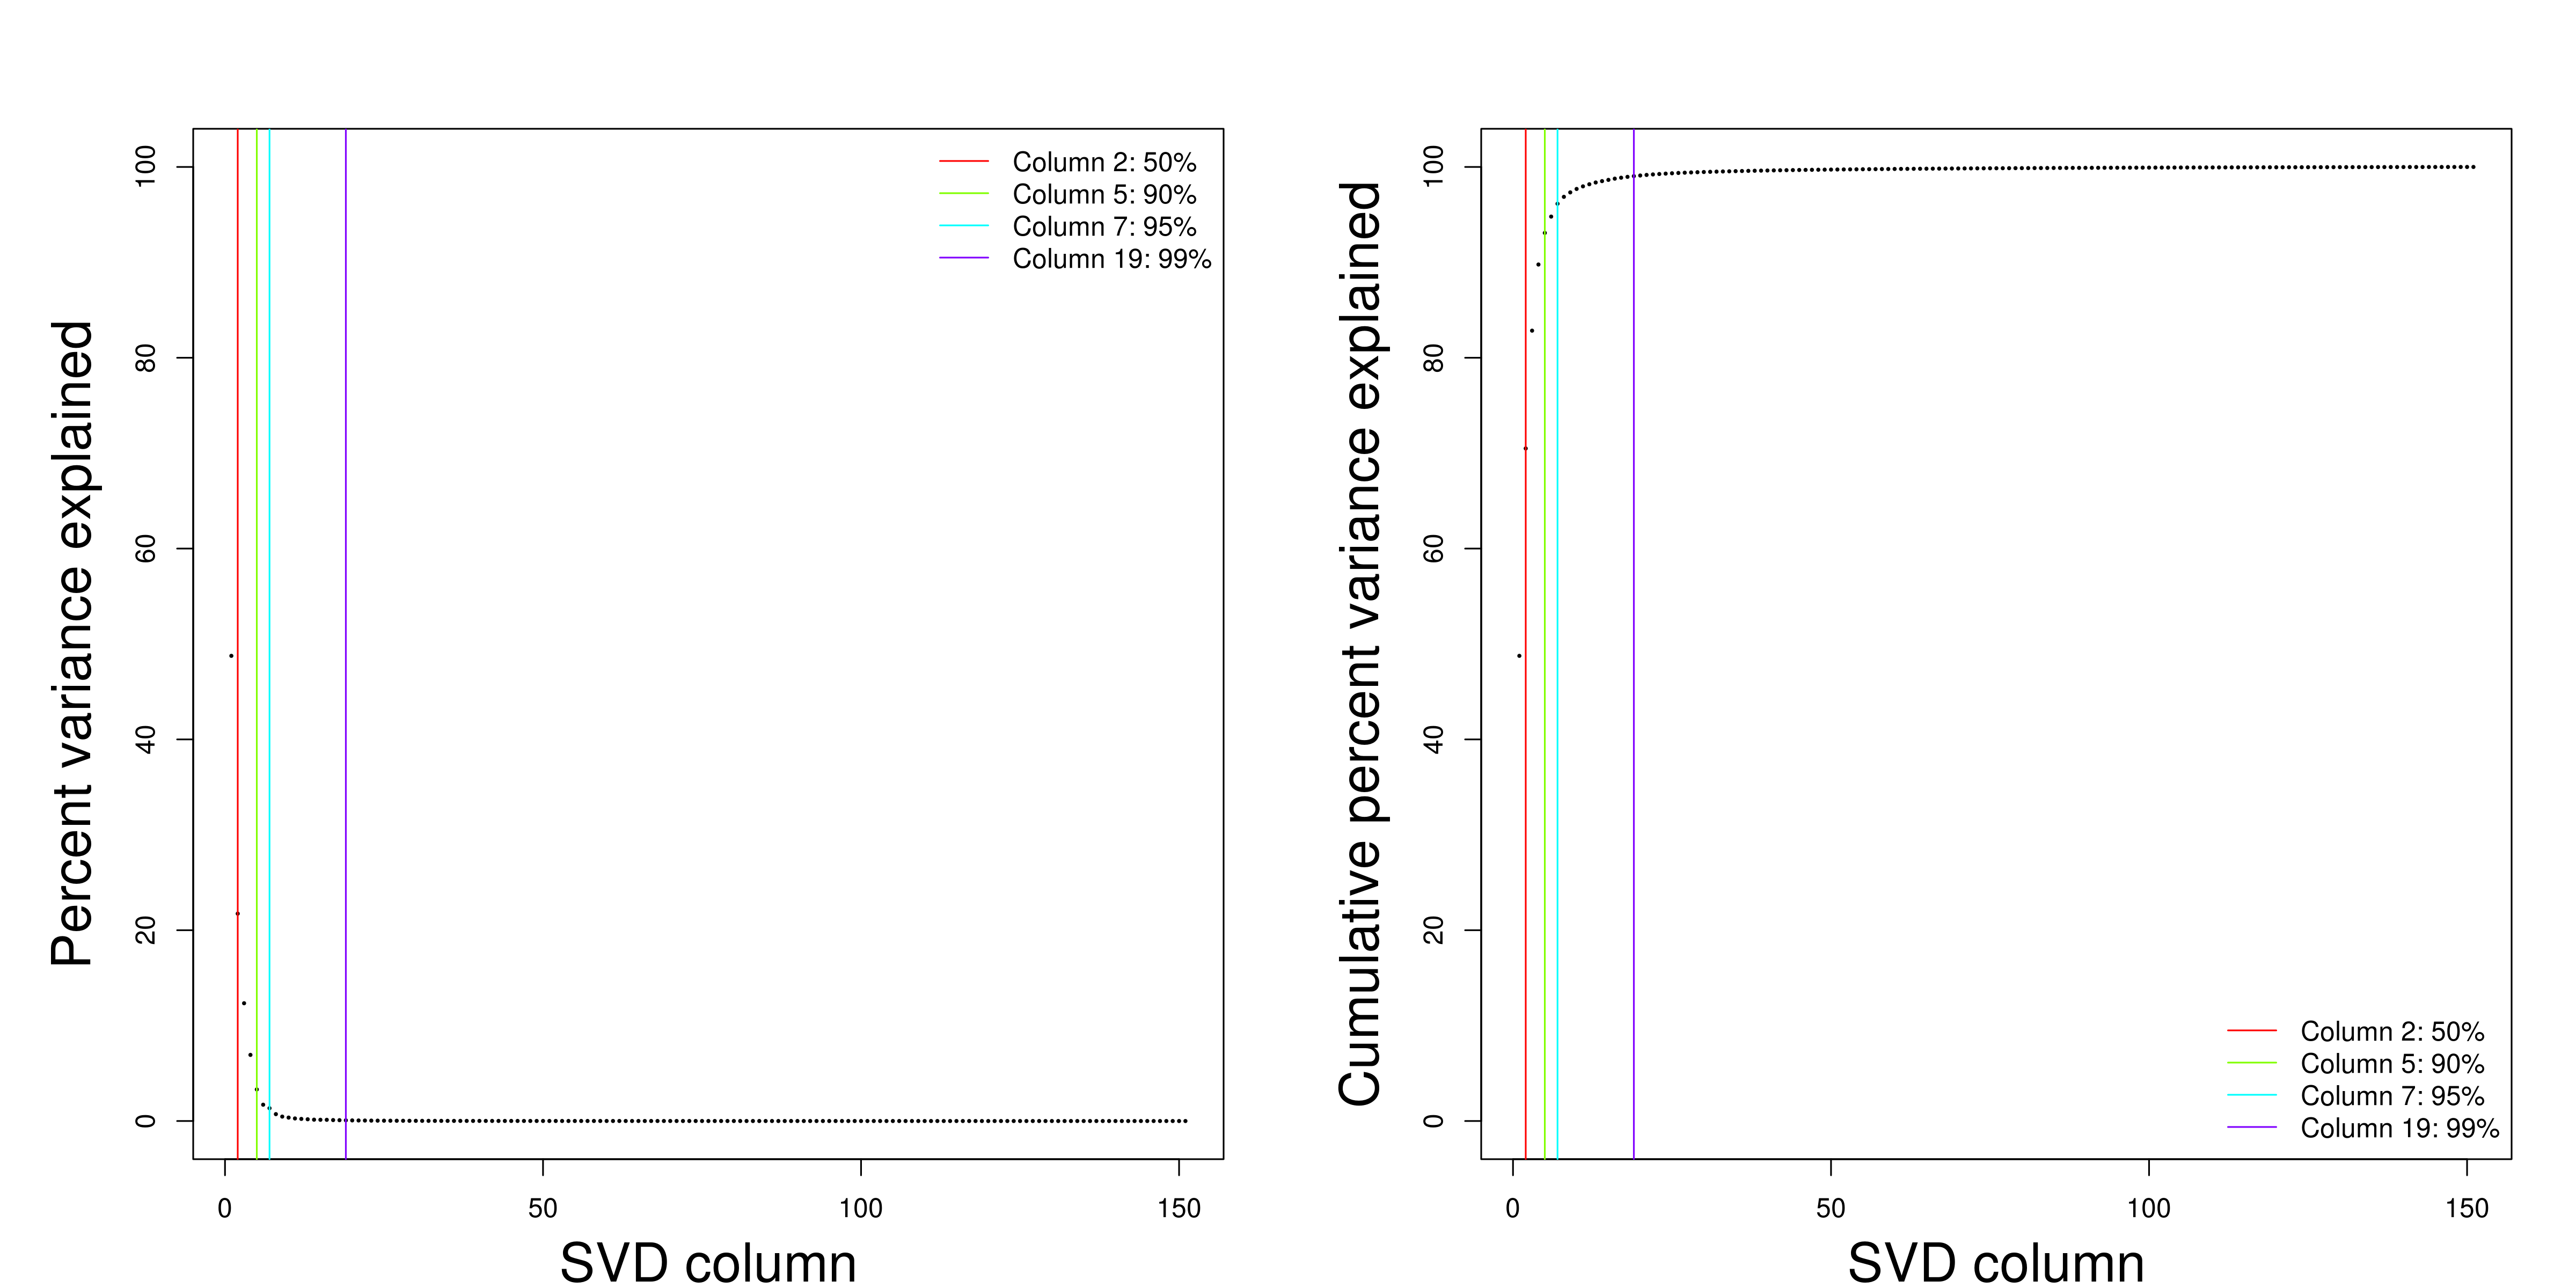
\includegraphics[width=15cm]{figures/fig-SVD}
\end{center}
\caption{Variance explained by successive LiDAR SVD singular vectors.}
\label{fig:SVD}
\end{figure}

Figure~\ref{fig:SVD} suggests that the first four singular vectors explain over 90\% of the signal variance. The code below plots the signal components described by these four singular vectors over the original signals.

\begin{Schunk}
\begin{Sinput}
> par(mfrow = c(2, 2), mar = c(4, 6, 4, 2))
> X.fit <- eof.fit(X, 4)
> for (i in 1:4) {
+     plot(X[i, ], 1:ncol(X), typ = "l", ylab = "Vertical (Canopy height)", 
+         xlab = "Standardized signal")
+     lines(X.fit[i, ], 1:ncol(X), col = "blue")
+ }
\end{Sinput}
\end{Schunk}

\begin{figure}
\begin{center}
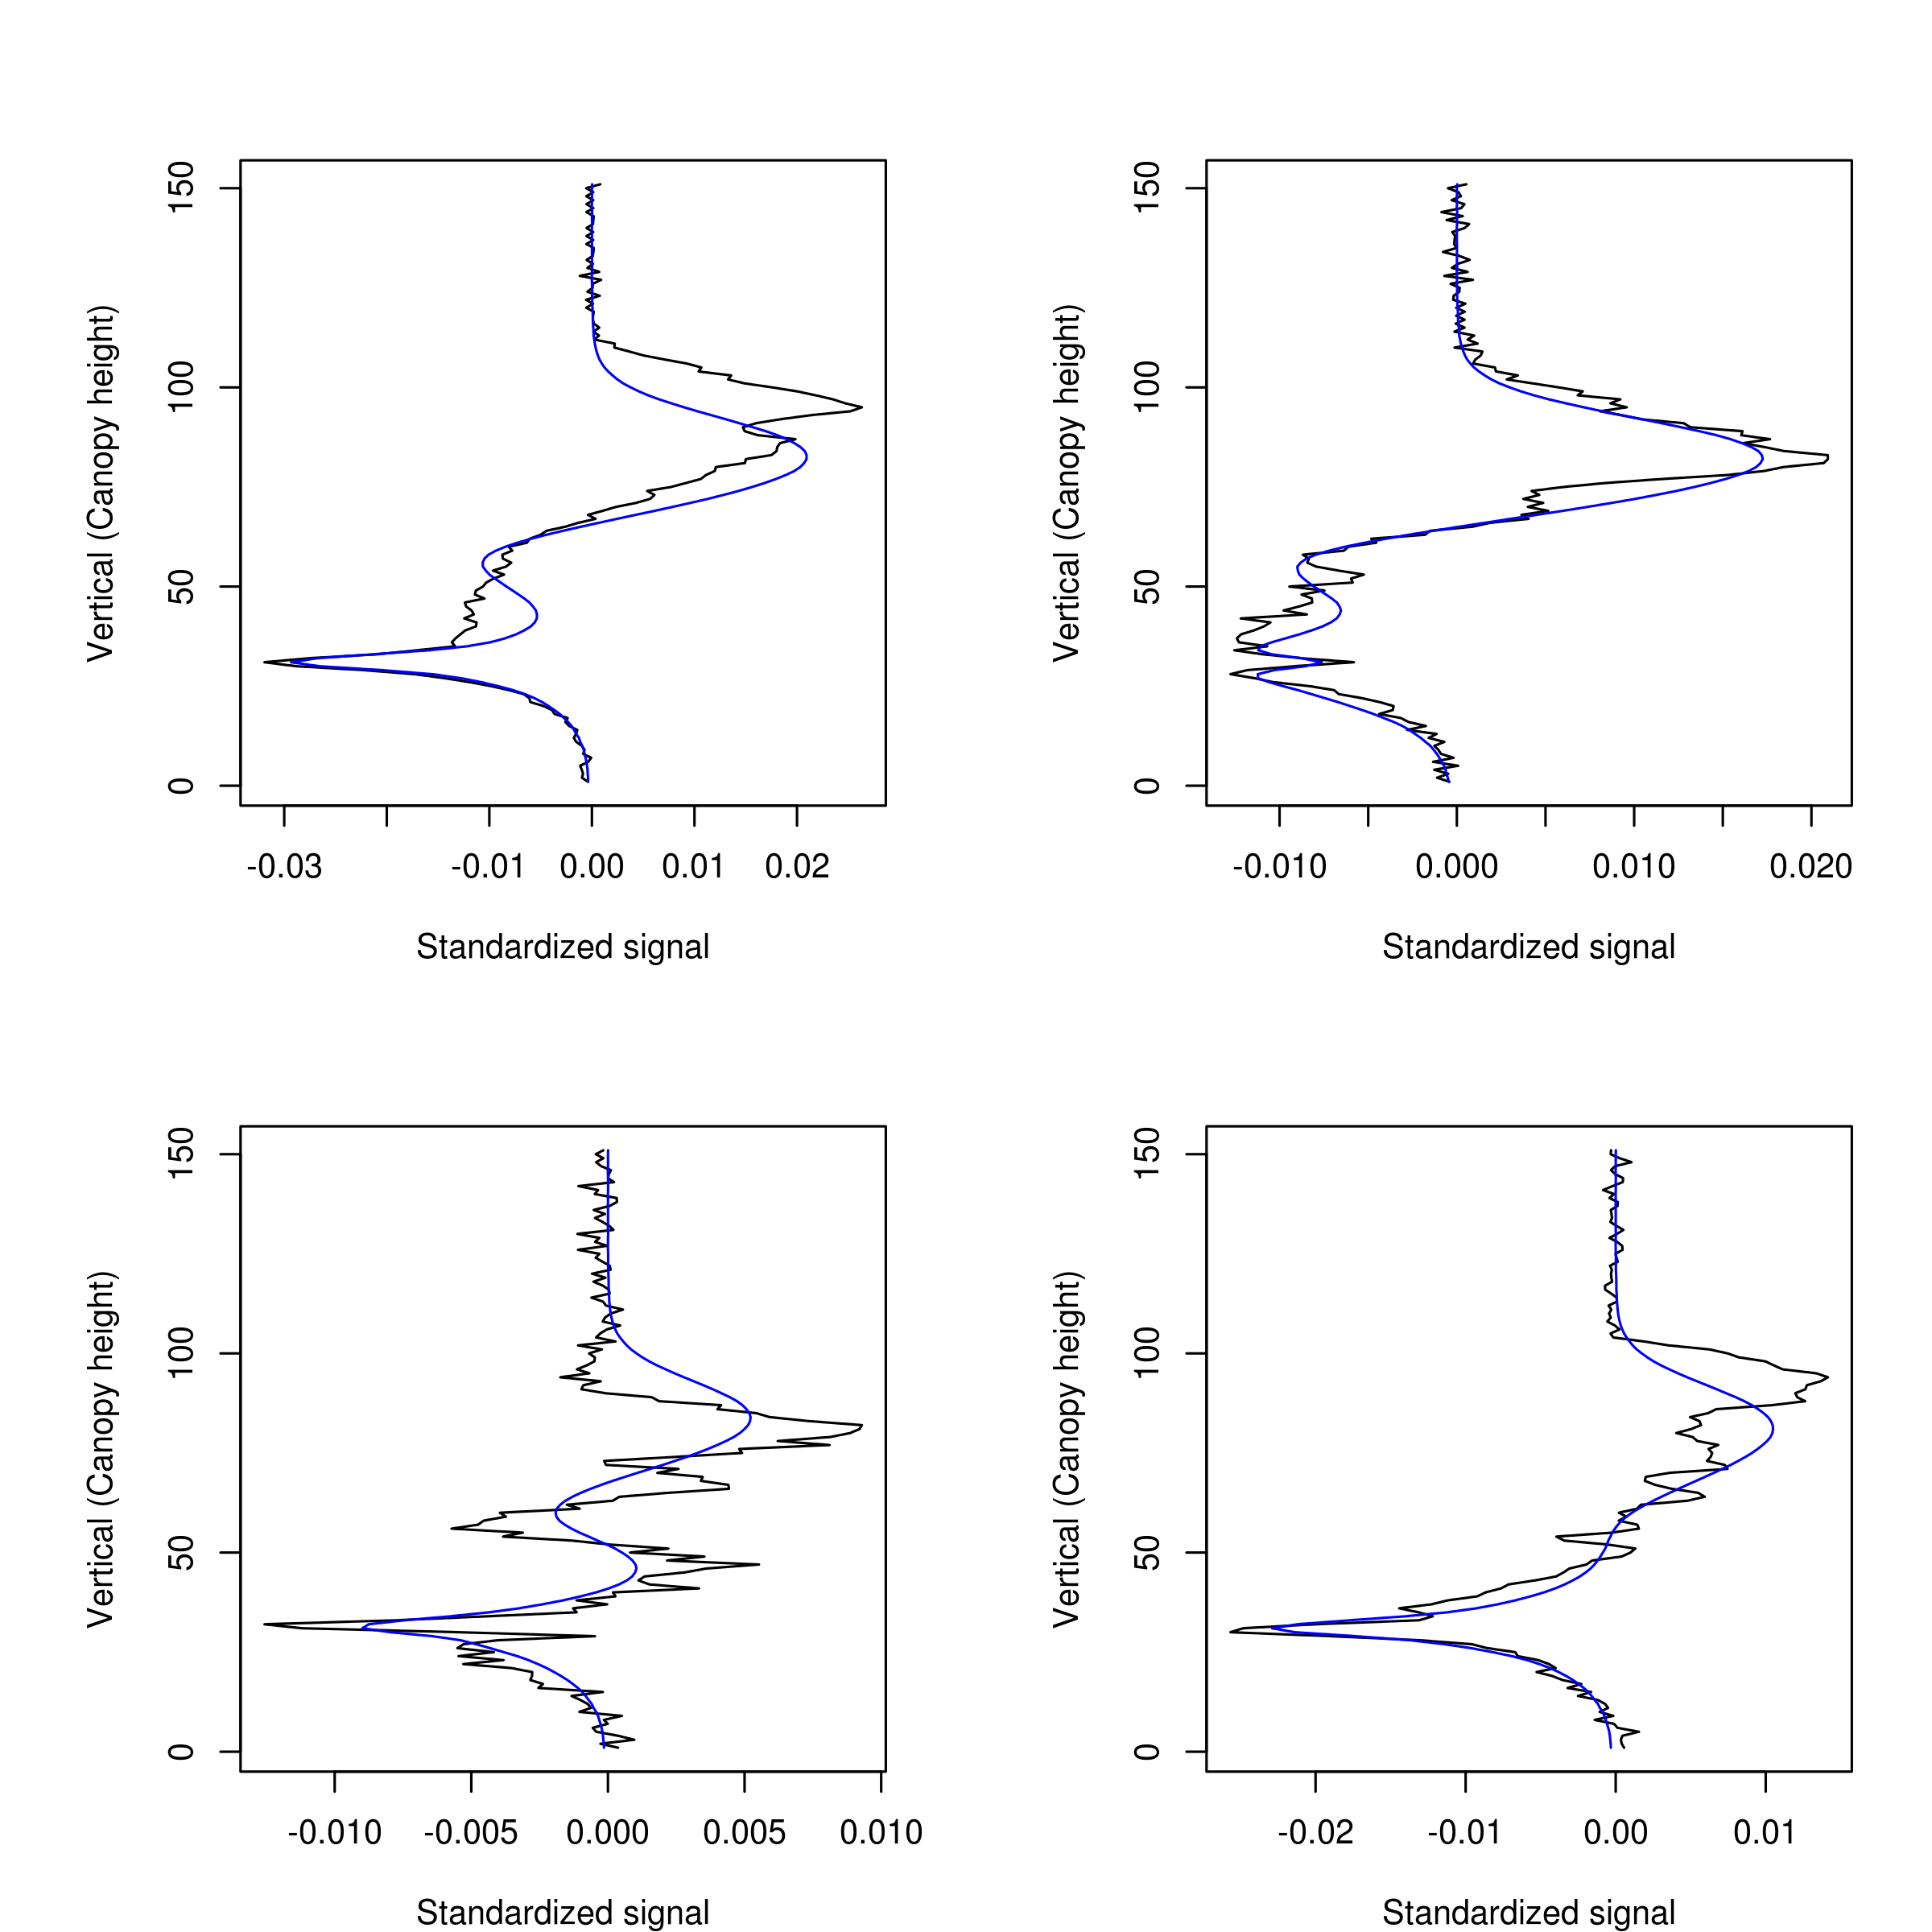
\includegraphics[width=15cm]{figures/fig-SVDFitted}
\end{center}
\caption{Four original LiDAR signals (black line) and first four SVD component reconstruction of the signals (blue line).}
\label{fig:SVDFitted}
\end{figure}

We can also look at a surface representation of these potential covariates Figure~\ref{fig:SVDSurf}. Here, we are only interested in selecting covariates useful for prediction; however, in other settings we might actually want a biological or forest structure understanding of what these components represent. In such cases it could be useful to consider Figure~\ref{fig:SVDSurf} in combination with inventory plot structure metrics and/or other remotely sensed data, e.g., high-resolution aerial images Figure~\ref{fig:Google}.

\begin{Schunk}
\begin{Sinput}
> lvis.coords <- lvis[, 1:2]
> Z <- eof(X, 4)
> z.1 <- mba.surf(cbind(lvis.coords, Z[, 1]), no.X = 200, no.Y = 200, 
+     h = 10, extend = TRUE)$xyz.est
> z.2 <- mba.surf(cbind(lvis.coords, Z[, 2]), no.X = 200, no.Y = 200, 
+     h = 10, extend = TRUE)$xyz.est
> z.3 <- mba.surf(cbind(lvis.coords, Z[, 3]), no.X = 200, no.Y = 200, 
+     h = 10, extend = TRUE)$xyz.est
> z.4 <- mba.surf(cbind(lvis.coords, Z[, 4]), no.X = 200, no.Y = 200, 
+     h = 10, extend = TRUE)$xyz.est
> par(mfrow = c(2, 2))
> image.plot(z.1, xaxs = "r", yaxs = "r", xlab = "", ylab = "Northing (m)")
> image.plot(z.2, xaxs = "r", yaxs = "r", xlab = "", ylab = "")
> image.plot(z.3, xaxs = "r", yaxs = "r", xlab = "Easting (m)", ylab = "Northing (m)")
> image.plot(z.4, xaxs = "r", yaxs = "r", xlab = "Easting (m)", ylab = "")
\end{Sinput}
\end{Schunk}

\begin{figure}
\begin{center}
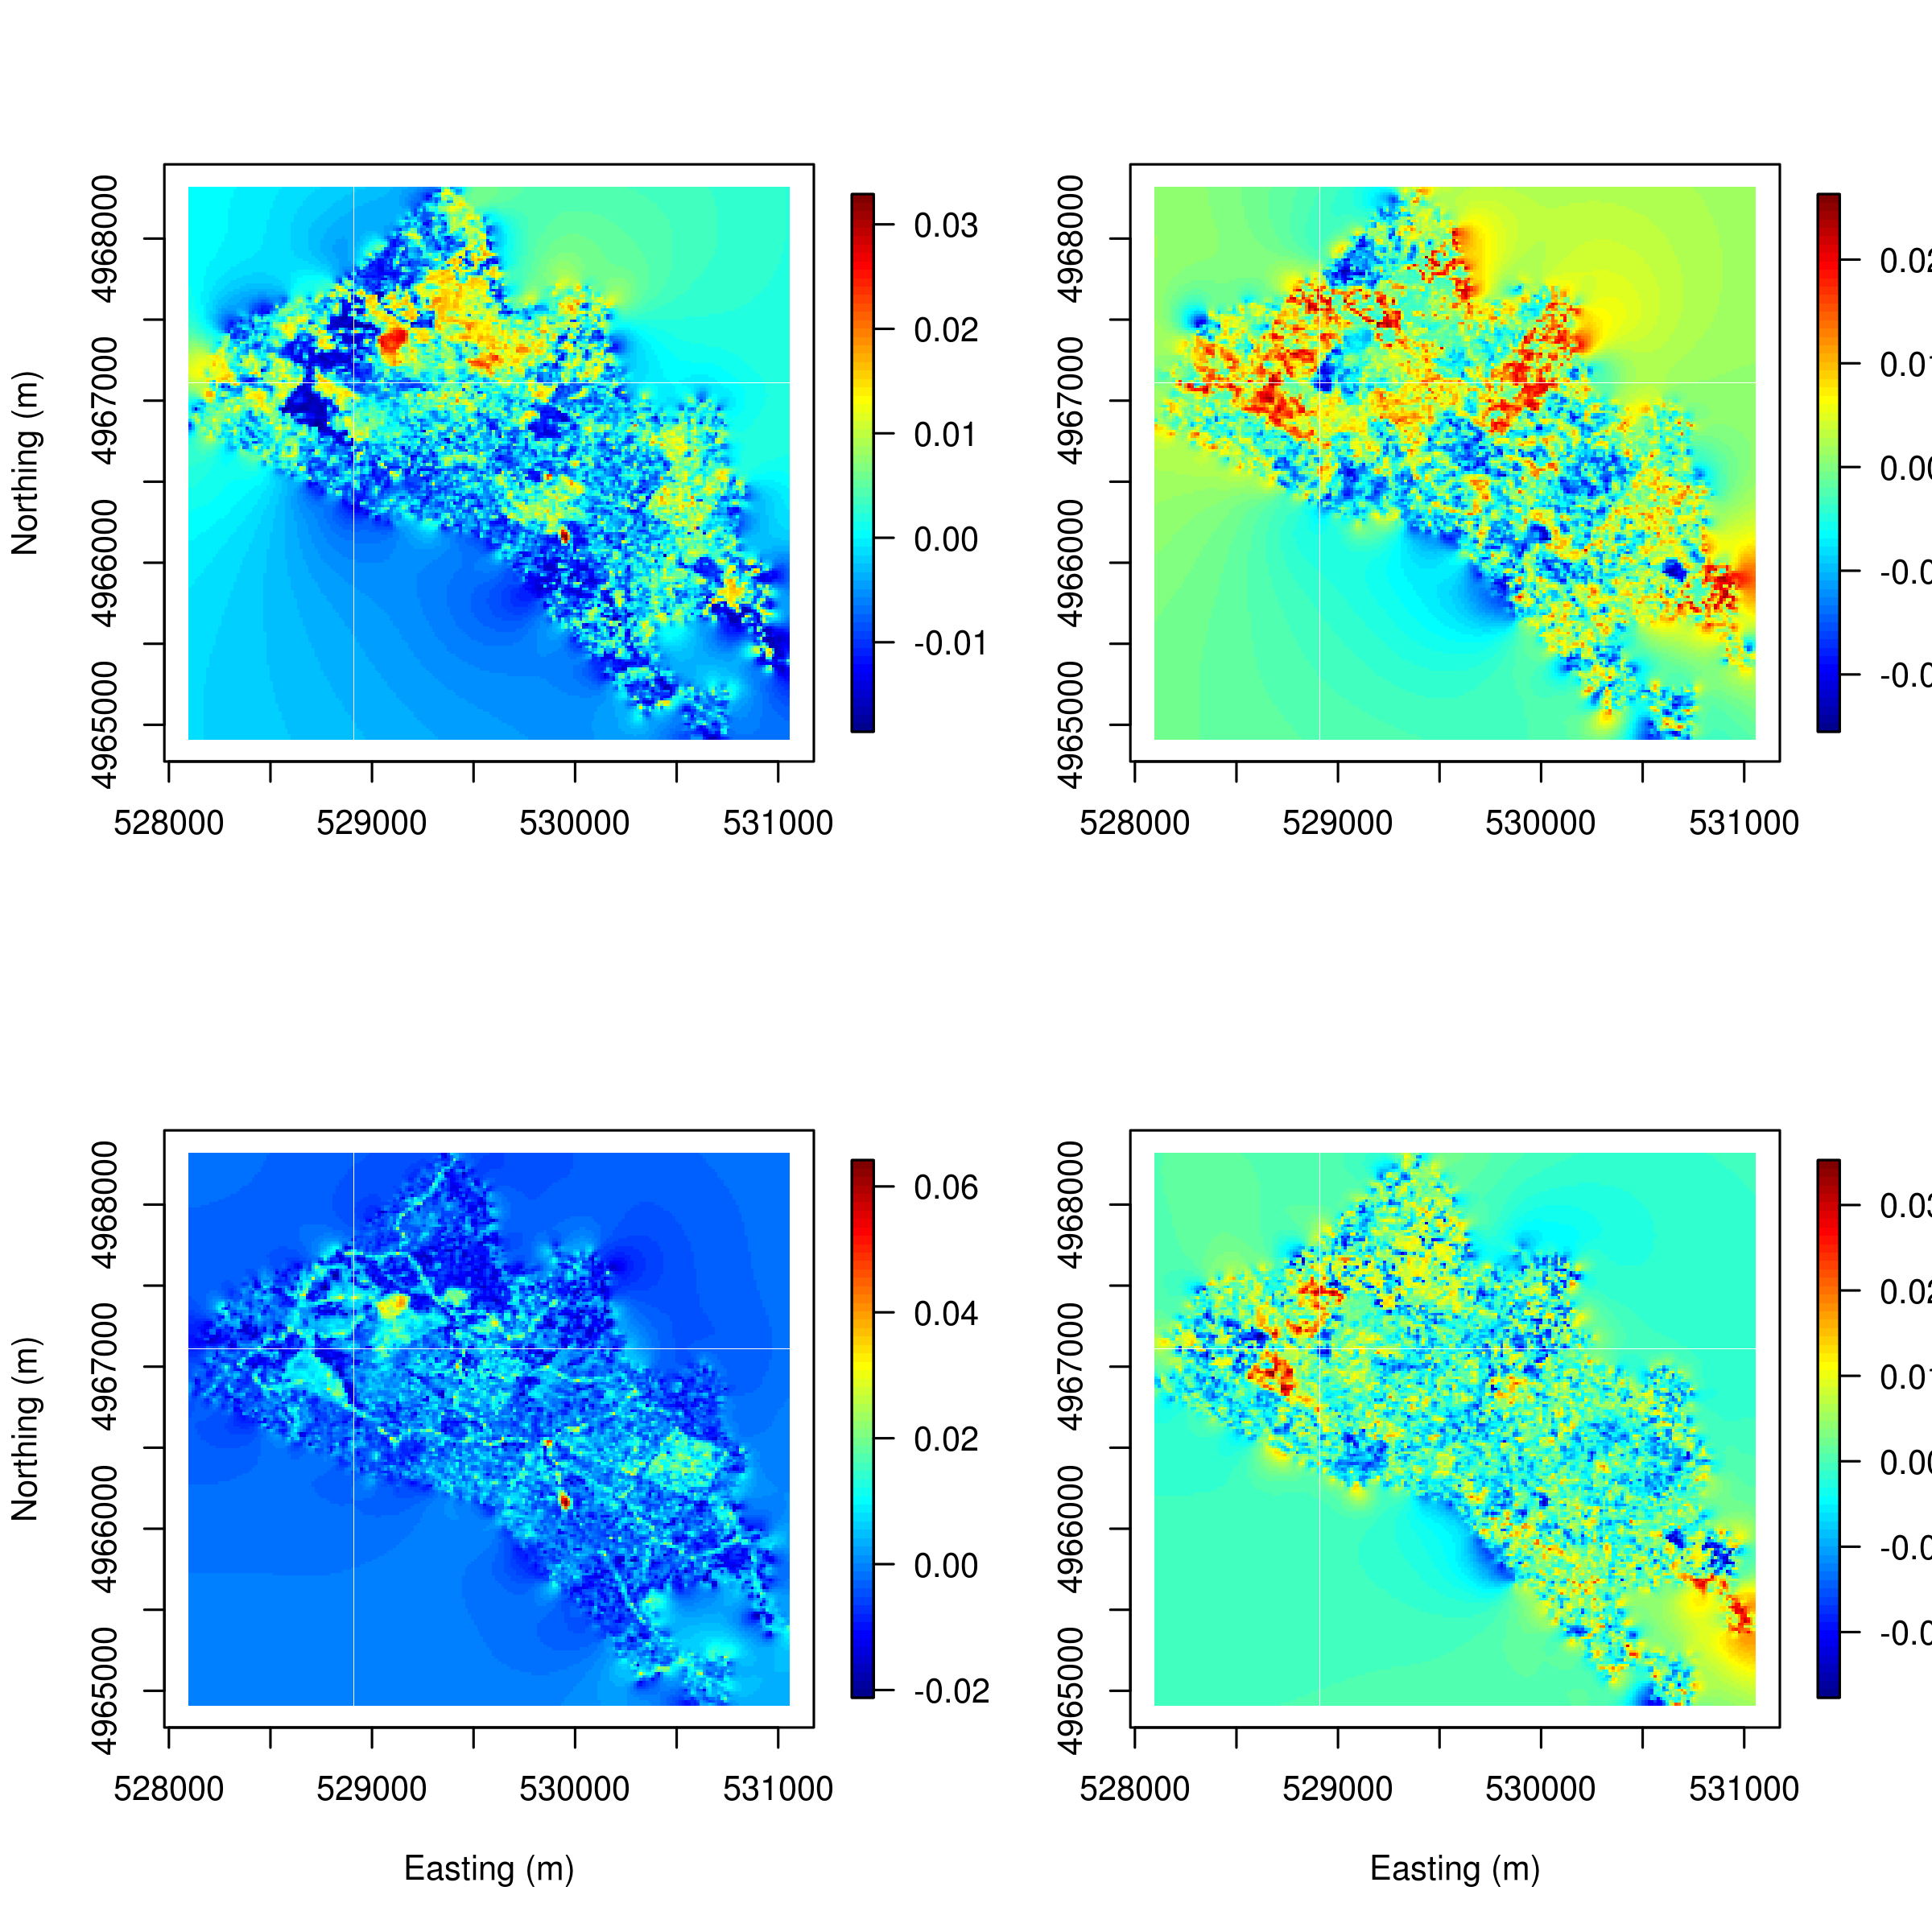
\includegraphics[width=15cm]{figures/fig-SVDSurf}
\end{center}
\caption{First four SVD component surfaces.}
\label{fig:SVDSurf}
\end{figure}

\begin{Schunk}
\begin{Sinput}
> proj4string(PEF.shp) <- CRS("+proj=utm +zone=18 +ellps=WGS84 +datum=WGS84 +units=m +no_defs")
> PEF.shp.LL <- spTransform(PEF.shp, CRS("+proj=longlat"))
> bounds <- bbox(PEF.shp.LL)
> img <- GetMap.bbox(bounds[1, ], bounds[2, ], maptype = "satellite")
\end{Sinput}
\begin{Soutput}
[1] "http://maps.google.com/maps/api/staticmap?center=44.8523225289668,-74.6258030343401&zoom=14&size=640x640&maptype=satellite&format=png32&sensor=true"
\end{Soutput}
\begin{Sinput}
> bounds <- img$BBOX
> img <- stack("MyTile.png")
> extent(img) = extent(bounds$ll[, 2], bounds$ur[, 2], bounds$ll[, 
+     1], bounds$ur[, 1])
> plotRGB(img)
> plot(PEF.shp.LL, add = TRUE, border = "yellow", usePolypath = FALSE)
\end{Sinput}
\end{Schunk}
\begin{figure}
\begin{center}
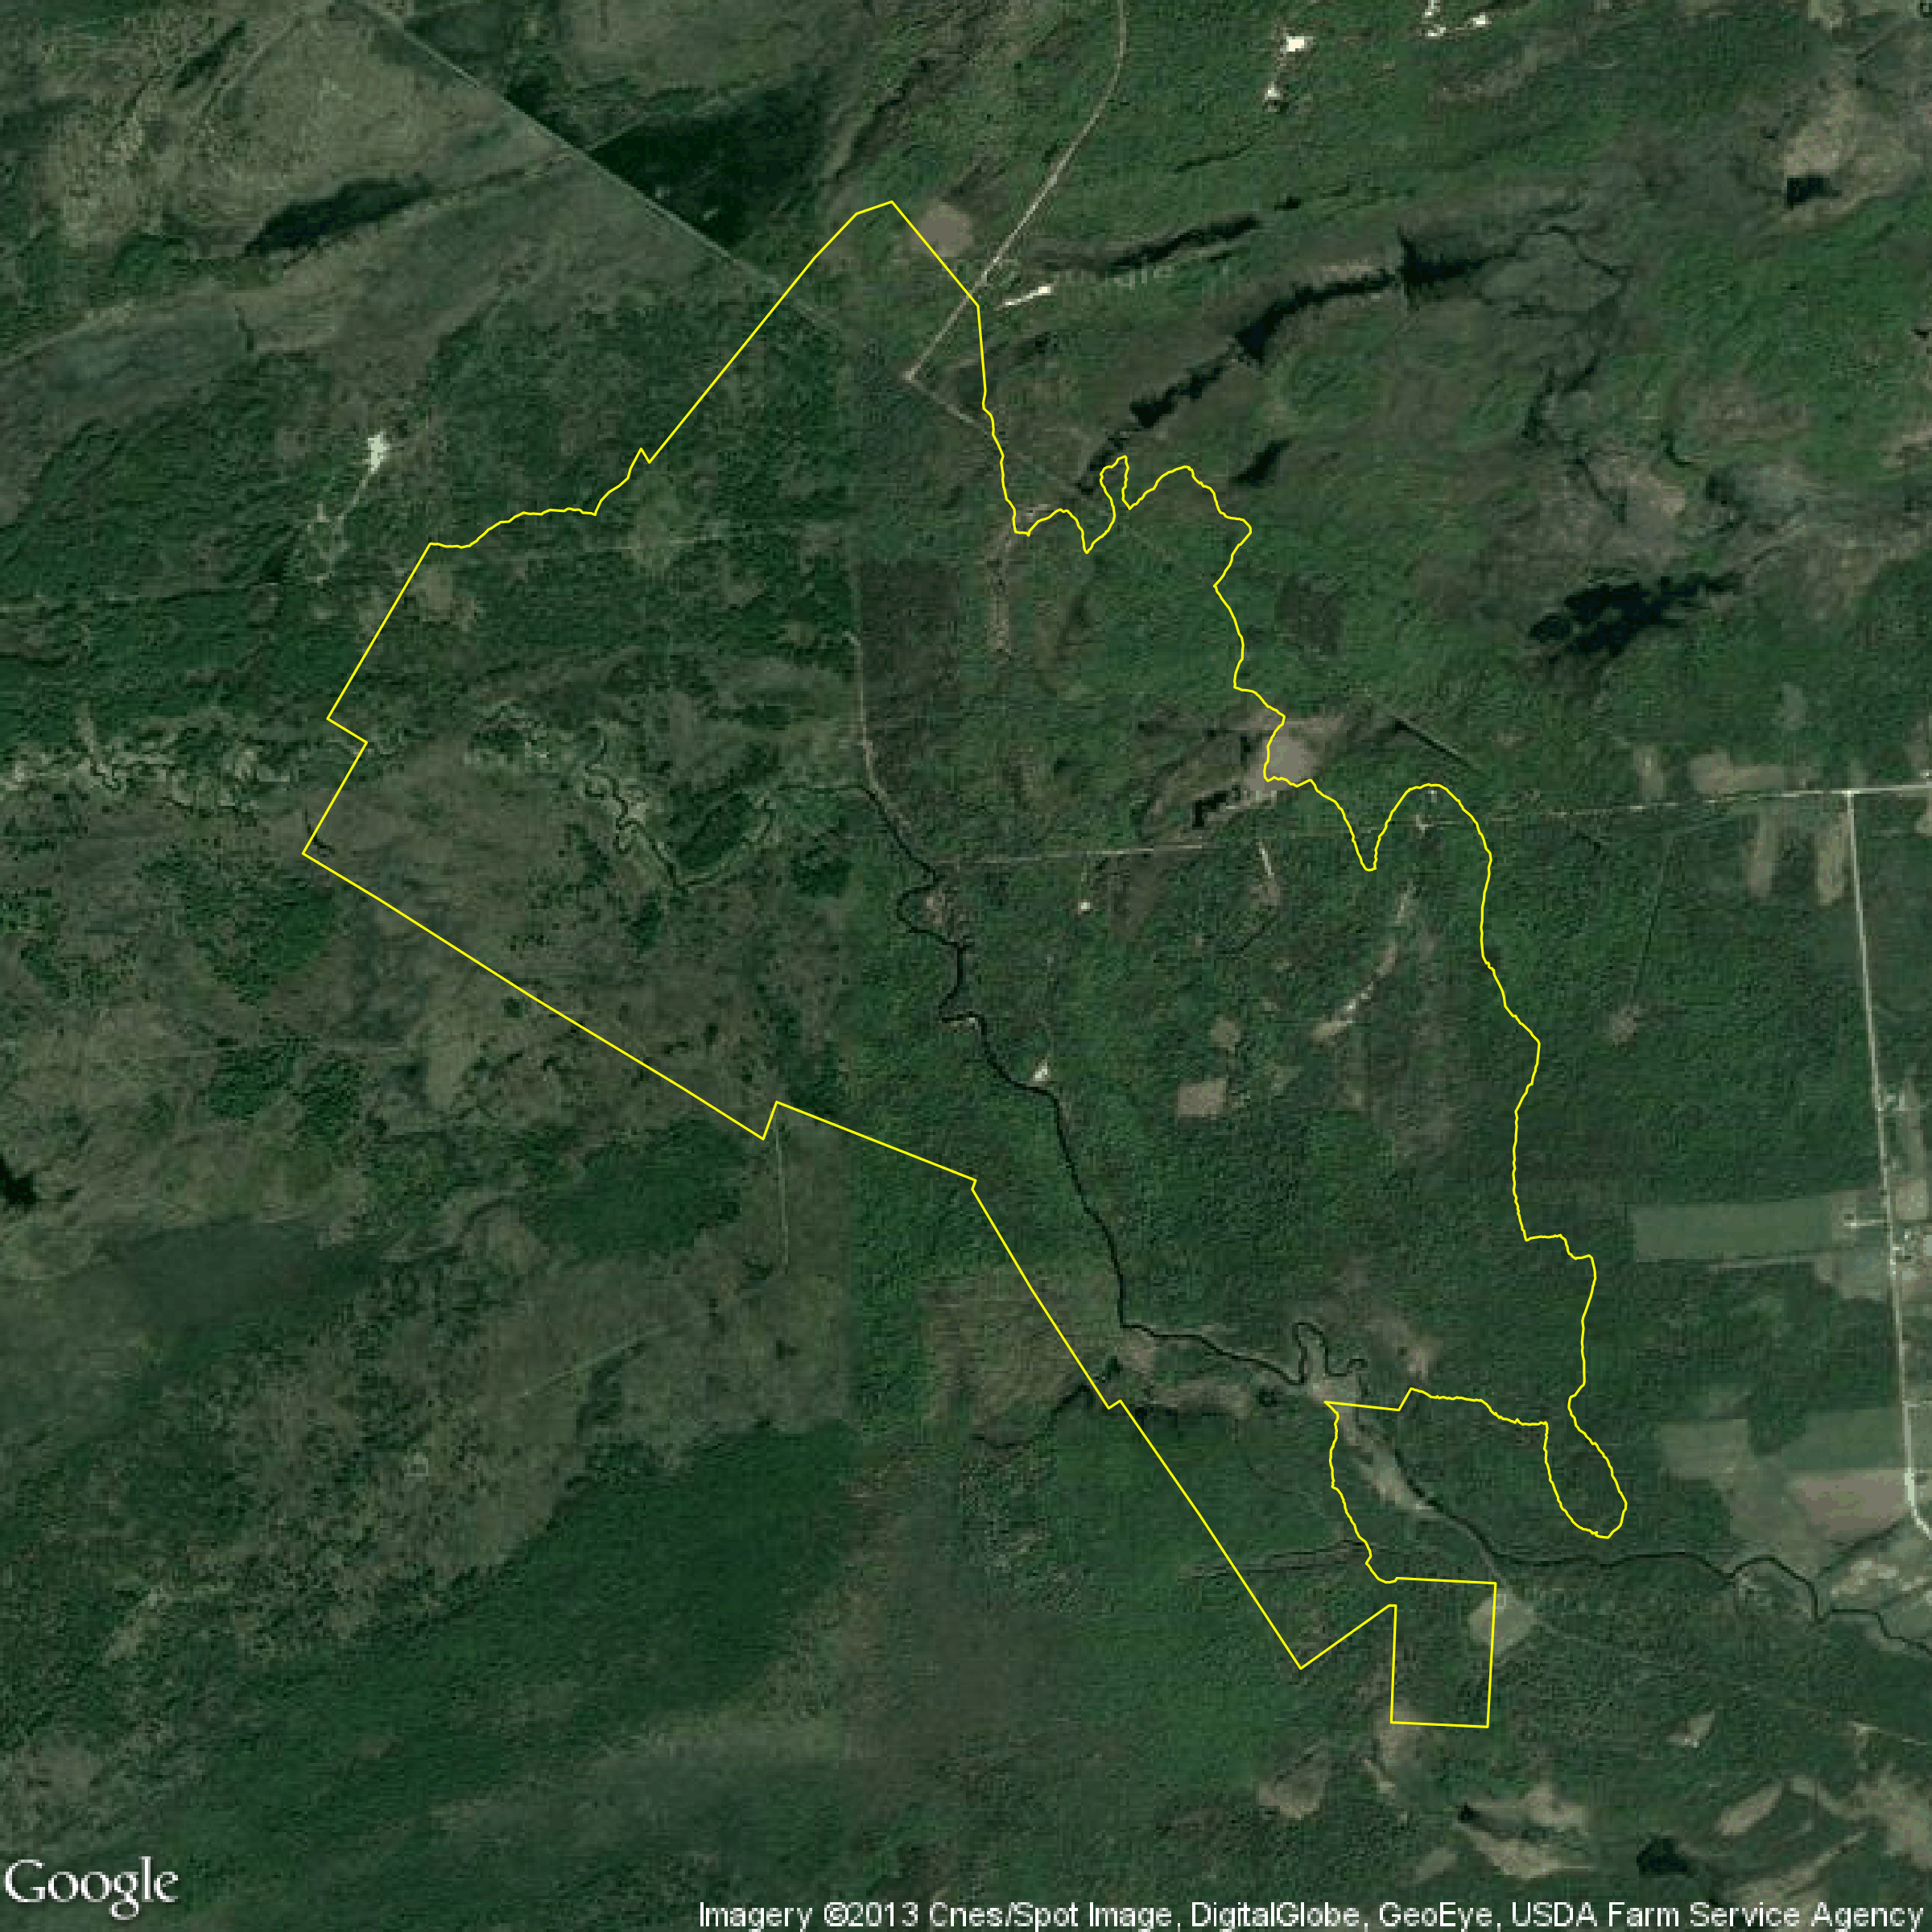
\includegraphics[width=10cm]{figures/fig-Google}
\end{center}
\caption{Google image of PEF.}
\label{fig:Google}
\end{figure}

\section{Exploratory data analysis}
In the code block below we match the inventory plots with SVD covariates derived from the nearest LiDAR signal, then regress biomass onto the set of covariates, then use \verb@mba.surf@ to make image plots of the residuals, Figure~\ref{fig:MBAResids}.

\begin{Schunk}
\begin{Sinput}
> PEF.plots.Z <- Z[ann(as.matrix(lvis.coords), as.matrix(coords))$knnIndexDist[, 
+     1], ]
\end{Sinput}
\begin{Soutput}
Target points completed: 
		100...200...300...400...
\end{Soutput}
\begin{Sinput}
> bio <- sqrt(PEF.plots$biomass.mg.ha)
> m <- lm(bio ~ PEF.plots.Z)
> summary(m)
\end{Sinput}
\begin{Soutput}
Call:
lm(formula = bio ~ PEF.plots.Z)

Residuals:
    Min      1Q  Median      3Q     Max 
-5.7752 -0.9775  0.1600  1.2460  5.6735 

Coefficients:
               Estimate Std. Error t value Pr(>|t|)    
(Intercept)    10.05107    0.09411 106.804  < 2e-16 ***
PEF.plots.Z1 -170.33901   10.45809 -16.288  < 2e-16 ***
PEF.plots.Z2  -93.70959   11.03247  -8.494 3.01e-16 ***
PEF.plots.Z3   -0.81924   11.50711  -0.071    0.943    
PEF.plots.Z4    4.88962    9.93443   0.492    0.623    
---
Signif. codes:  0 ‘***’ 0.001 ‘**’ 0.01 ‘*’ 0.05 ‘.’ 0.1 ‘ ’ 1 

Residual standard error: 1.933 on 446 degrees of freedom
Multiple R-squared: 0.4019,	Adjusted R-squared: 0.3965 
F-statistic: 74.91 on 4 and 446 DF,  p-value: < 2.2e-16 
\end{Soutput}
\begin{Sinput}
> bio.resid <- resid(m)
> resid.surf <- mba.surf(cbind(coords, bio.resid), no.X = 200, no.Y = 200, 
+     extend = FALSE)$xyz.est
> image.plot(resid.surf, xaxs = "r", yaxs = "r", main = "Square-root metric tons of biomass residuals", 
+     xlab = "Easting (m)", ylab = "Northing (m)")
\end{Sinput}
\end{Schunk}

\begin{figure}
\begin{center}
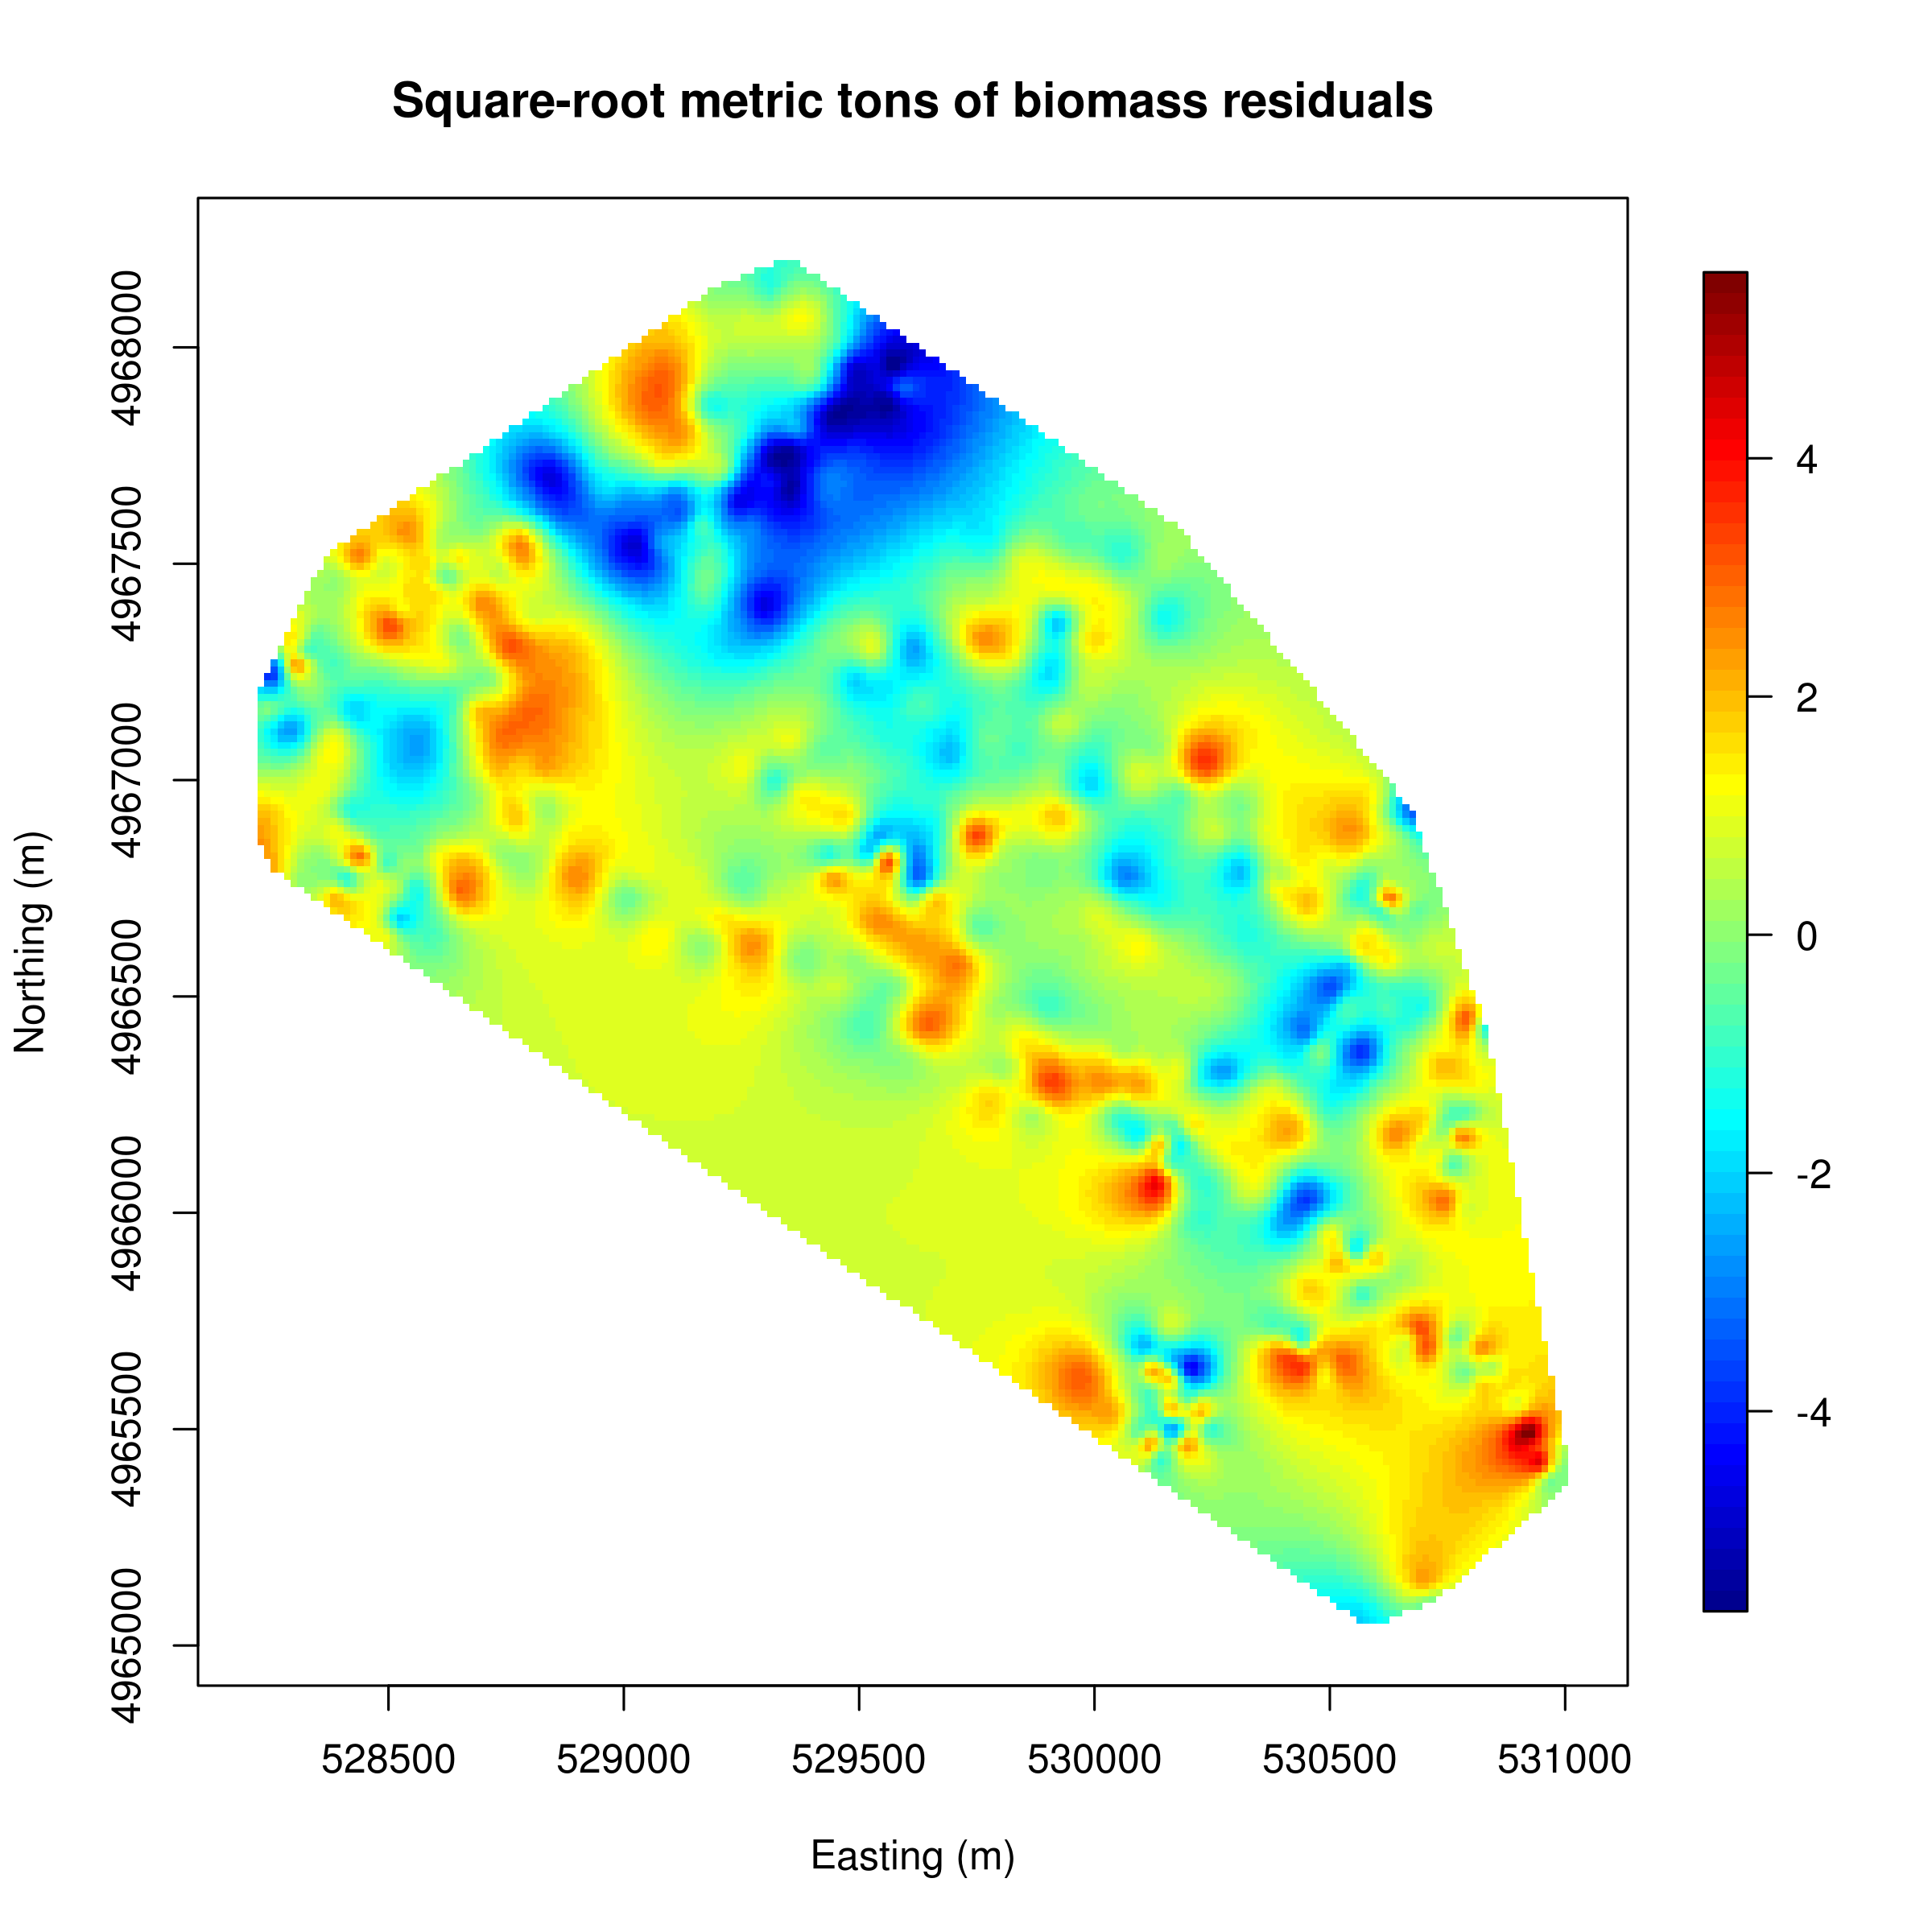
\includegraphics[width=10cm]{figures/fig-MBAResids}
\end{center}
\caption{Interpolation of square-root metric tons of biomass residuals using a Multilevel B-spline.}
\label{fig:MBAResids}
\end{figure}

The residual image plot in Figure~\ref{fig:MBAResids} suggests that there is spatial dependence even after accounting for the covariates. These patterns can be more formally examined using empirical semivariograms.  In the code block below, we first fit an exponential variogram model to transformed biomass then fit a second variogram model to the regression residuals. The resulting variograms are offered in Figure~\ref{fig:geoRVariog}. Here the upper and lower horizontal lines are the \emph{sill} and \emph{nugget}, respectively, and the vertical line is the effective range (i.e., that distance at which the correlation drops to 0.05).

\begin{Schunk}
\begin{Sinput}
> max.dist <- 0.5 * max(iDist(coords))
> bins <- 15
> vario.bio <- variog(coords = coords, data = bio, uvec = (seq(0, 
+     max.dist, length = bins)))
\end{Sinput}
\begin{Soutput}
variog: computing omnidirectional variogram
\end{Soutput}
\begin{Sinput}
> fit.bio <- variofit(vario.bio, ini.cov.pars = c(5, 500), cov.model = "exponential", 
+     minimisation.function = "nls", weights = "equal")
\end{Sinput}
\begin{Soutput}
variofit: covariance model used is exponential 
variofit: weights used: equal 
variofit: minimisation function used: nls 
\end{Soutput}
\begin{Sinput}
> vario.bio.resid <- variog(coords = coords, data = bio.resid, uvec = (seq(0, 
+     max.dist, length = bins)))
\end{Sinput}
\begin{Soutput}
variog: computing omnidirectional variogram
\end{Soutput}
\begin{Sinput}
> fit.bio.resid <- variofit(vario.bio.resid, ini.cov.pars = c(3, 500), 
+     cov.model = "exponential", minimisation.function = "nls", weights = "equal")
\end{Sinput}
\begin{Soutput}
variofit: covariance model used is exponential 
variofit: weights used: equal 
variofit: minimisation function used: nls 
\end{Soutput}
\begin{Sinput}
> par(mfrow = c(1, 2))
> plot(vario.bio, main = "Square-root metric tons of biomass")
> lines(fit.bio)
> abline(h = fit.bio$nugget, col = "blue")
> abline(h = fit.bio$cov.pars[1] + fit.bio$nugget, col = "green")
> abline(v = -log(0.05) * fit.bio$cov.pars[2], col = "red3")
> plot(vario.bio.resid, main = "Square-root metric tons of biomass residuals")
> lines(fit.bio.resid)
> abline(h = fit.bio.resid$nugget, col = "blue")
> abline(h = fit.bio.resid$cov.pars[1] + fit.bio.resid$nugget, col = "green")
> abline(v = -log(0.05) * fit.bio.resid$cov.pars[2], col = "red3")
\end{Sinput}
\end{Schunk}

\begin{figure}
\begin{center}
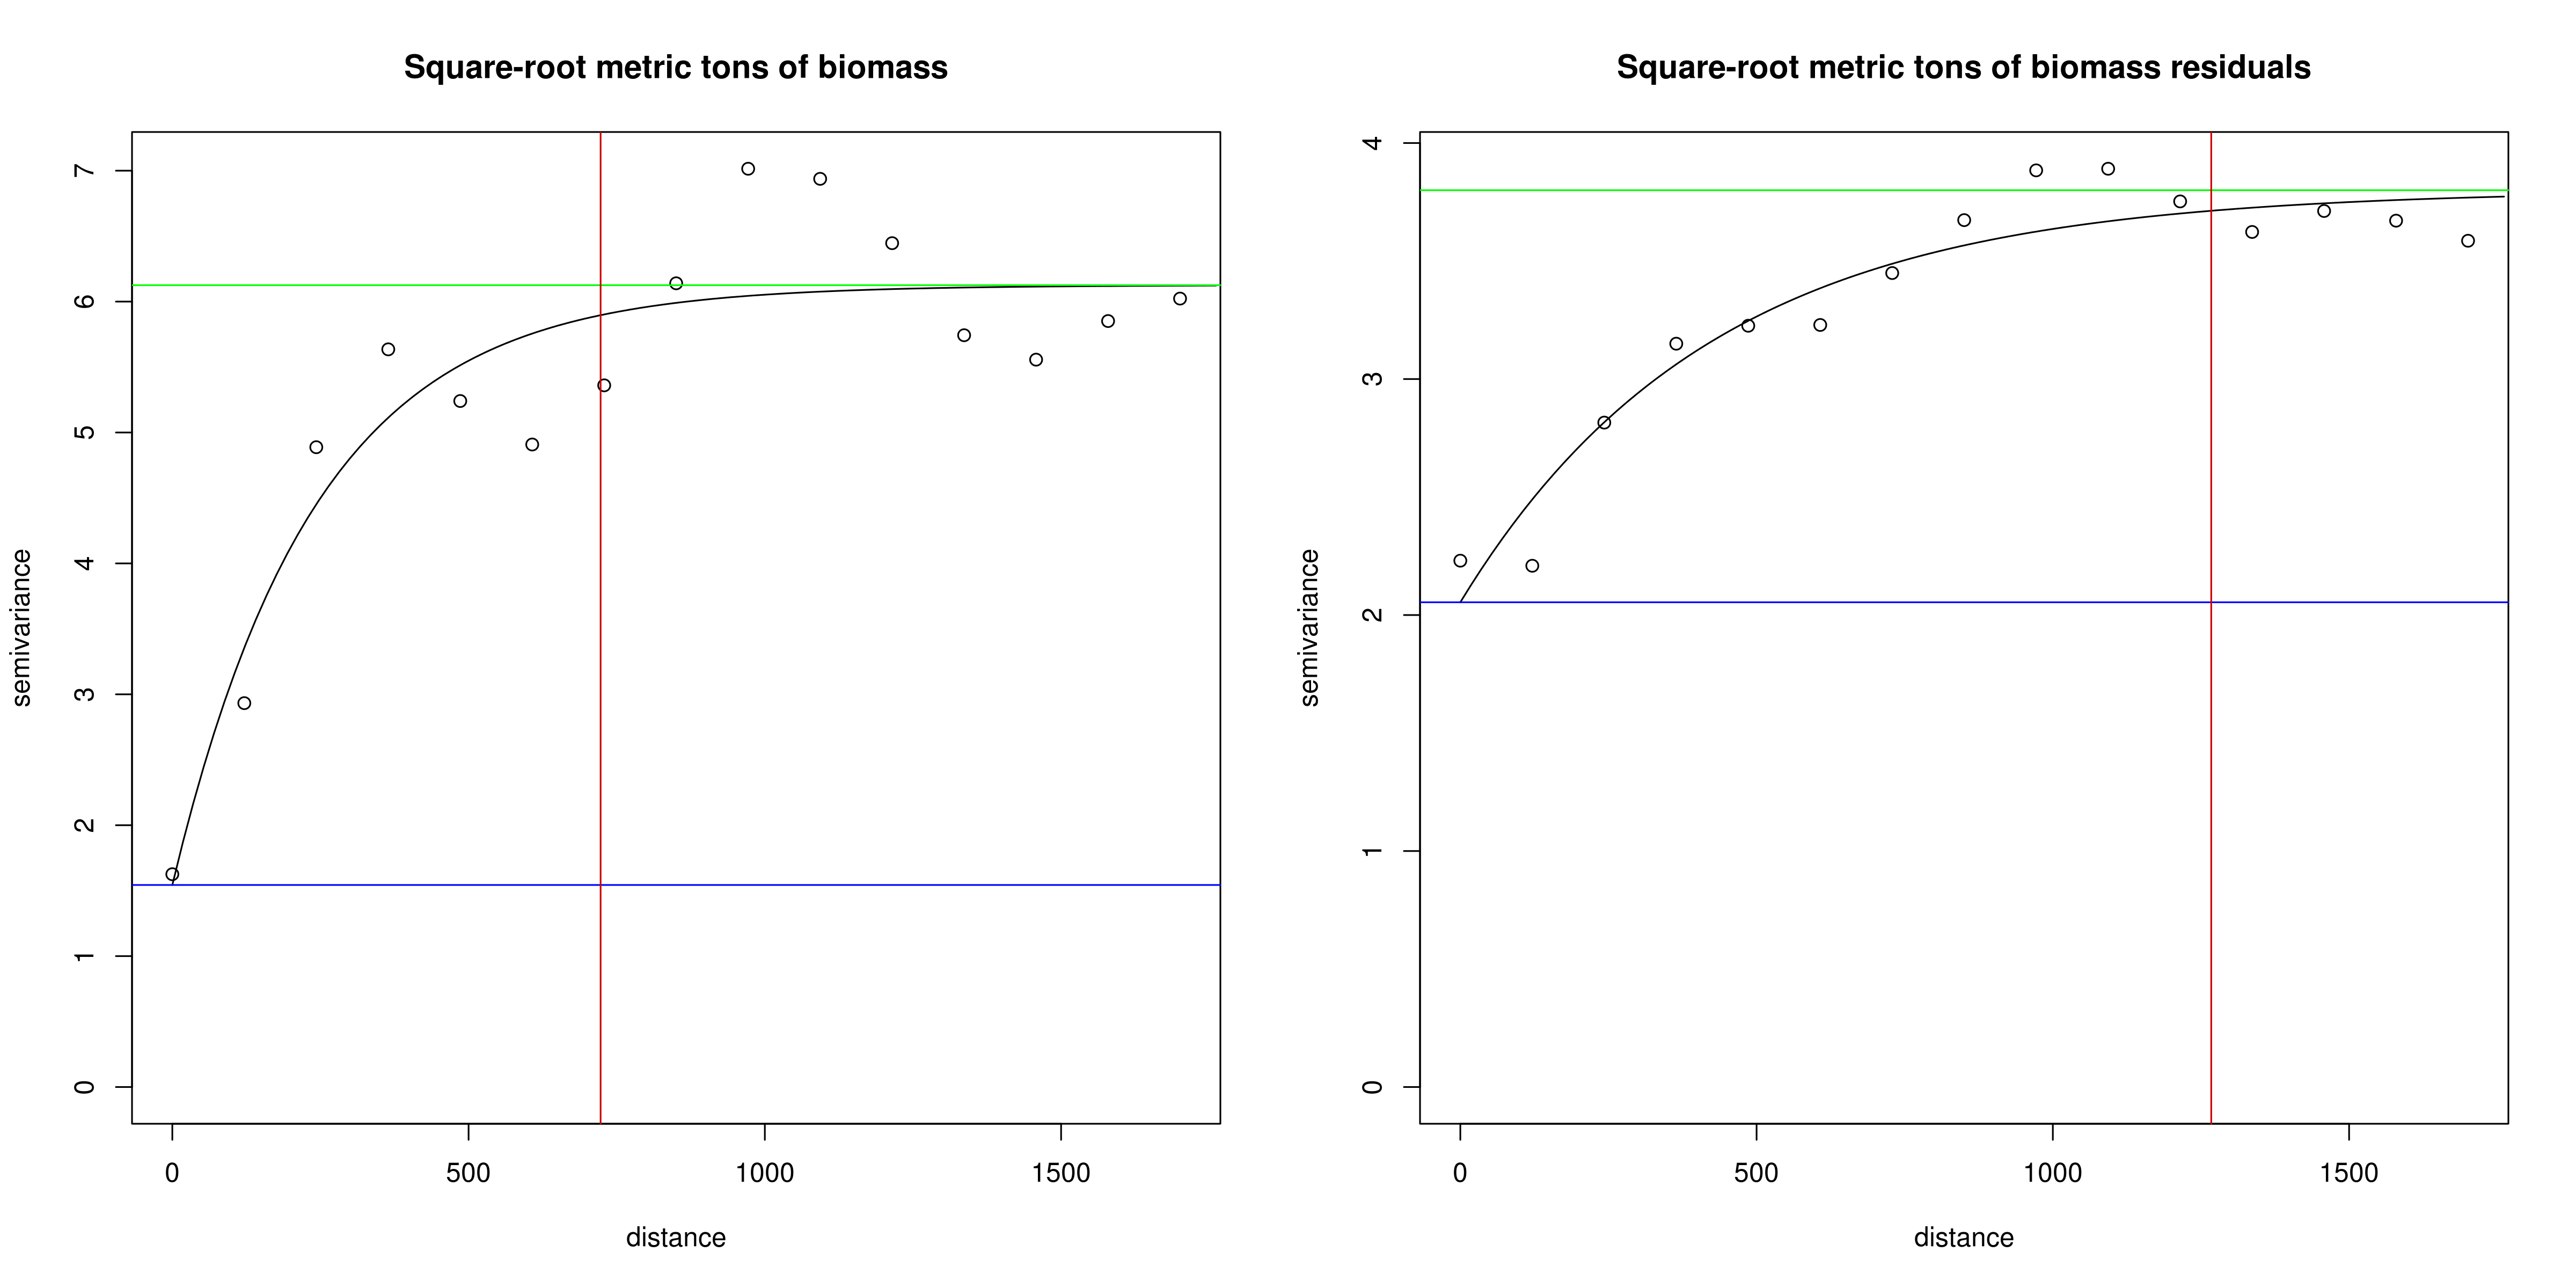
\includegraphics[width=16cm]{figures/fig-geoRVariog}
\end{center}
\caption{Isotropic semivariograms for log metric tons of biomass and residuals from a linear regression.}
\label{fig:geoRVariog}
\end{figure}

Figure~\ref{fig:geoRVariog} corroborates what is shown in the image plots. Specifically, there is substantial spatial dependence in biomass across the inventory plots and that this dependence persists, but to a lesser degree, after accounting for the predictor variables. Therefore, we expect that both the predictor variables and spatial proximity to inventory plots will improve prediction.

\section{Fitting spatial regression models}
The empirical semivariograms estimates of the partial sill, $\sigma^2$, nugget, $\tau^2$, and range $\phi$ provide good starting values to use in the \pkg{spBayes} univariate spatial regression function \verb@spLM@. For brevity, we only take 2000 MCMC sample in the code block below.

\begin{Schunk}
\begin{Sinput}
> n.samples <- 2000
> starting <- list(phi = 3/1000, sigma.sq = 2, tau.sq = 2)
> tuning <- list(phi = 0.5, sigma.sq = 0.01, tau.sq = 0.01)
> p <- ncol(PEF.plots.Z) + 1
> priors <- list(beta.Norm = list(rep(0, p), diag(1e+06, p)), phi.Unif = c(3/max.dist, 
+     3/10), sigma.sq.IG = c(2, 2), tau.sq.IG = c(2, 2))
> cov.model <- "exponential"
> m.1 <- spLM(bio ~ PEF.plots.Z, coords = as.matrix(coords), starting = starting, 
+     knots = c(10, 10), tuning = tuning, priors = priors, cov.model = cov.model, 
+     n.samples = n.samples, n.report = 1000)
\end{Sinput}
\begin{Soutput}
----------------------------------------
	General model description
----------------------------------------
Model fit with 451 observations.

Number of covariates 5 (including intercept if specified).

Using the exponential spatial correlation model.

Using modified predictive process with 100 knots.

Number of MCMC samples 2000.

Priors and hyperpriors:
	beta normal:
	mu:	0.000	0.000	0.000	0.000	0.000	
	cov:
	1000000.000	0.000	0.000	0.000	0.000	
	0.000	1000000.000	0.000	0.000	0.000	
	0.000	0.000	1000000.000	0.000	0.000	
	0.000	0.000	0.000	1000000.000	0.000	
	0.000	0.000	0.000	0.000	1000000.000	

	sigma.sq IG hyperpriors shape=2.00000 and scale=2.00000
	tau.sq IG hyperpriors shape=2.00000 and scale=2.00000
	phi Unif hyperpriors a=0.00176 and b=0.30000
-------------------------------------------------
		Sampling
-------------------------------------------------
Sampled: 1000 of 2000, 50.00%
Report interval Metrop. Acceptance rate: 44.60%
Overall Metrop. Acceptance rate: 44.60%
-------------------------------------------------
Sampled: 2000 of 2000, 100.00%
Report interval Metrop. Acceptance rate: 49.70%
Overall Metrop. Acceptance rate: 47.15%
-------------------------------------------------
\end{Soutput}
\end{Schunk}

The call to \verb@spLM@ provides samples from $\btheta = \{\sigma^2, \tau^2, \phi\}$. If \verb@cov.model@ is ``matern'', then $\btheta$ includes the spatial smoothness $\nu$. 

If it is difficult to maintain an acceptable Metropolis algorithm acceptance rate or one desires a fully automated call to \verb@spLM@, the \verb@amcmc@ argument can be used as illustrated below. 
\begin{Schunk}
\begin{Sinput}
> n.batch <- 40
> batch.length <- 50
> n.samples <- n.batch * batch.length
> m.2 <- spLM(bio ~ PEF.plots.Z, coords = as.matrix(coords), starting = starting, 
+     knots = c(10, 10), tuning = tuning, priors = priors, cov.model = cov.model, 
+     amcmc = list(n.batch = n.batch, batch.length = batch.length, 
+         accept.rate = 0.43), n.report = 10)
\end{Sinput}
\begin{Soutput}
----------------------------------------
	General model description
----------------------------------------
Model fit with 451 observations.

Number of covariates 5 (including intercept if specified).

Using the exponential spatial correlation model.

Using modified predictive process with 100 knots.

Using adaptive MCMC.

	Number of batches 40.
	Batch length 50.
	Target acceptance rate 0.43000.

Priors and hyperpriors:
	beta normal:
	mu:	0.000	0.000	0.000	0.000	0.000	
	cov:
	1000000.000	0.000	0.000	0.000	0.000	
	0.000	1000000.000	0.000	0.000	0.000	
	0.000	0.000	1000000.000	0.000	0.000	
	0.000	0.000	0.000	1000000.000	0.000	
	0.000	0.000	0.000	0.000	1000000.000	

	sigma.sq IG hyperpriors shape=2.00000 and scale=2.00000
	tau.sq IG hyperpriors shape=2.00000 and scale=2.00000
	phi Unif hyperpriors a=0.00176 and b=0.30000
-------------------------------------------------
		Sampling
-------------------------------------------------
Batch: 10 of 40, 25.00%
	parameter	acceptance	tuning
	sigma.sq	58.0%		0.11052
	tau.sq		80.0%		0.11052
	phi		54.0%		0.76600
-------------------------------------------------
Batch: 20 of 40, 50.00%
	parameter	acceptance	tuning
	sigma.sq	66.0%		0.12214
	tau.sq		68.0%		0.12214
	phi		58.0%		0.84656
-------------------------------------------------
Batch: 30 of 40, 75.00%
	parameter	acceptance	tuning
	sigma.sq	60.0%		0.13499
	tau.sq		64.0%		0.13499
	phi		60.0%		0.89891
-------------------------------------------------
Batch: 40 of 40, 100.00%
	parameter	acceptance	tuning
	sigma.sq	54.0%		0.14918
	tau.sq		74.0%		0.14918
	phi		64.0%		0.97378
-------------------------------------------------
\end{Soutput}
\end{Schunk}

\begin{Schunk}
\begin{Sinput}
> theta.samps <- mcmc.list(m.1$p.theta.samples, m.2$p.theta.samples)
> plot(theta.samps, density = FALSE)
\end{Sinput}
\end{Schunk}

\begin{Schunk}
\begin{Sinput}
> beta.samps <- mcmc.list(m.1$p.beta.samples, m.2$p.beta.samples)
> plot(beta.samps, density = FALSE)
\end{Sinput}
\end{Schunk}

\begin{figure}
\begin{center}
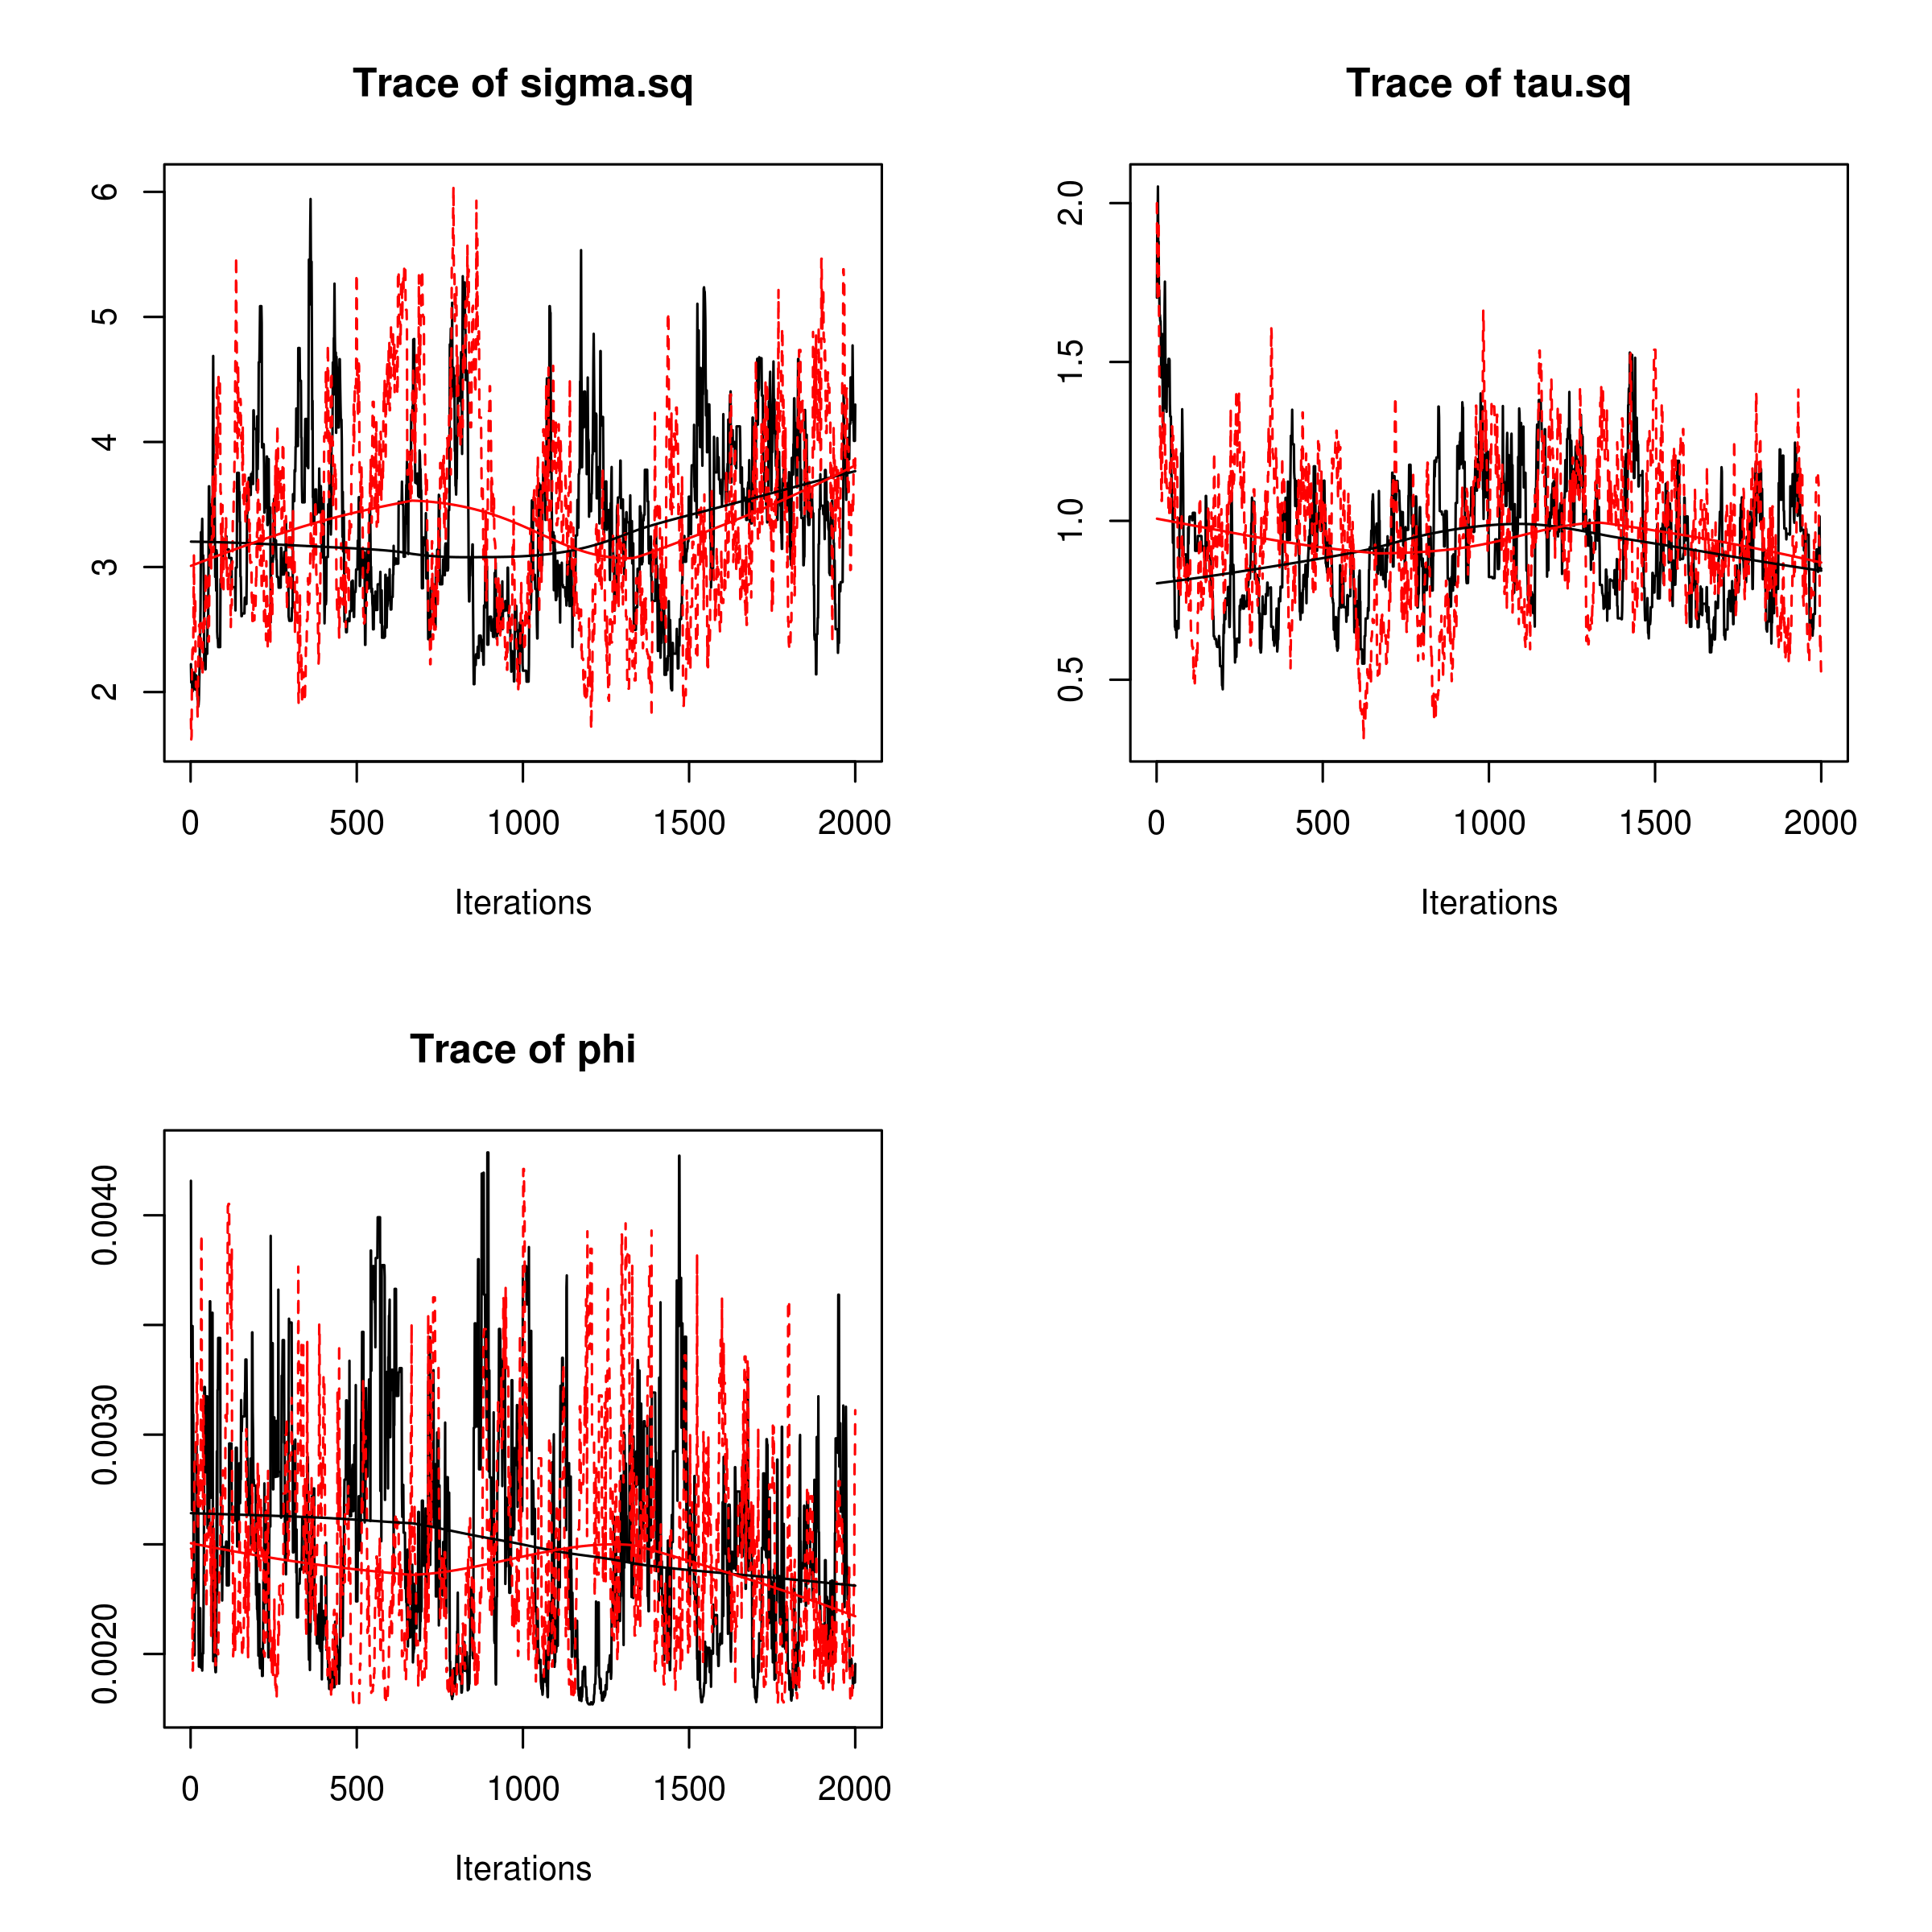
\includegraphics[width=12cm]{figures/fig-thetaSamples}
\end{center}
\caption{MCMC trace plots of spatial parameters, $\sigma^2$, $\tau^2$, and $\phi$.}
\label{fig:thetaSamples}
\end{figure}

\begin{figure}
\begin{center}
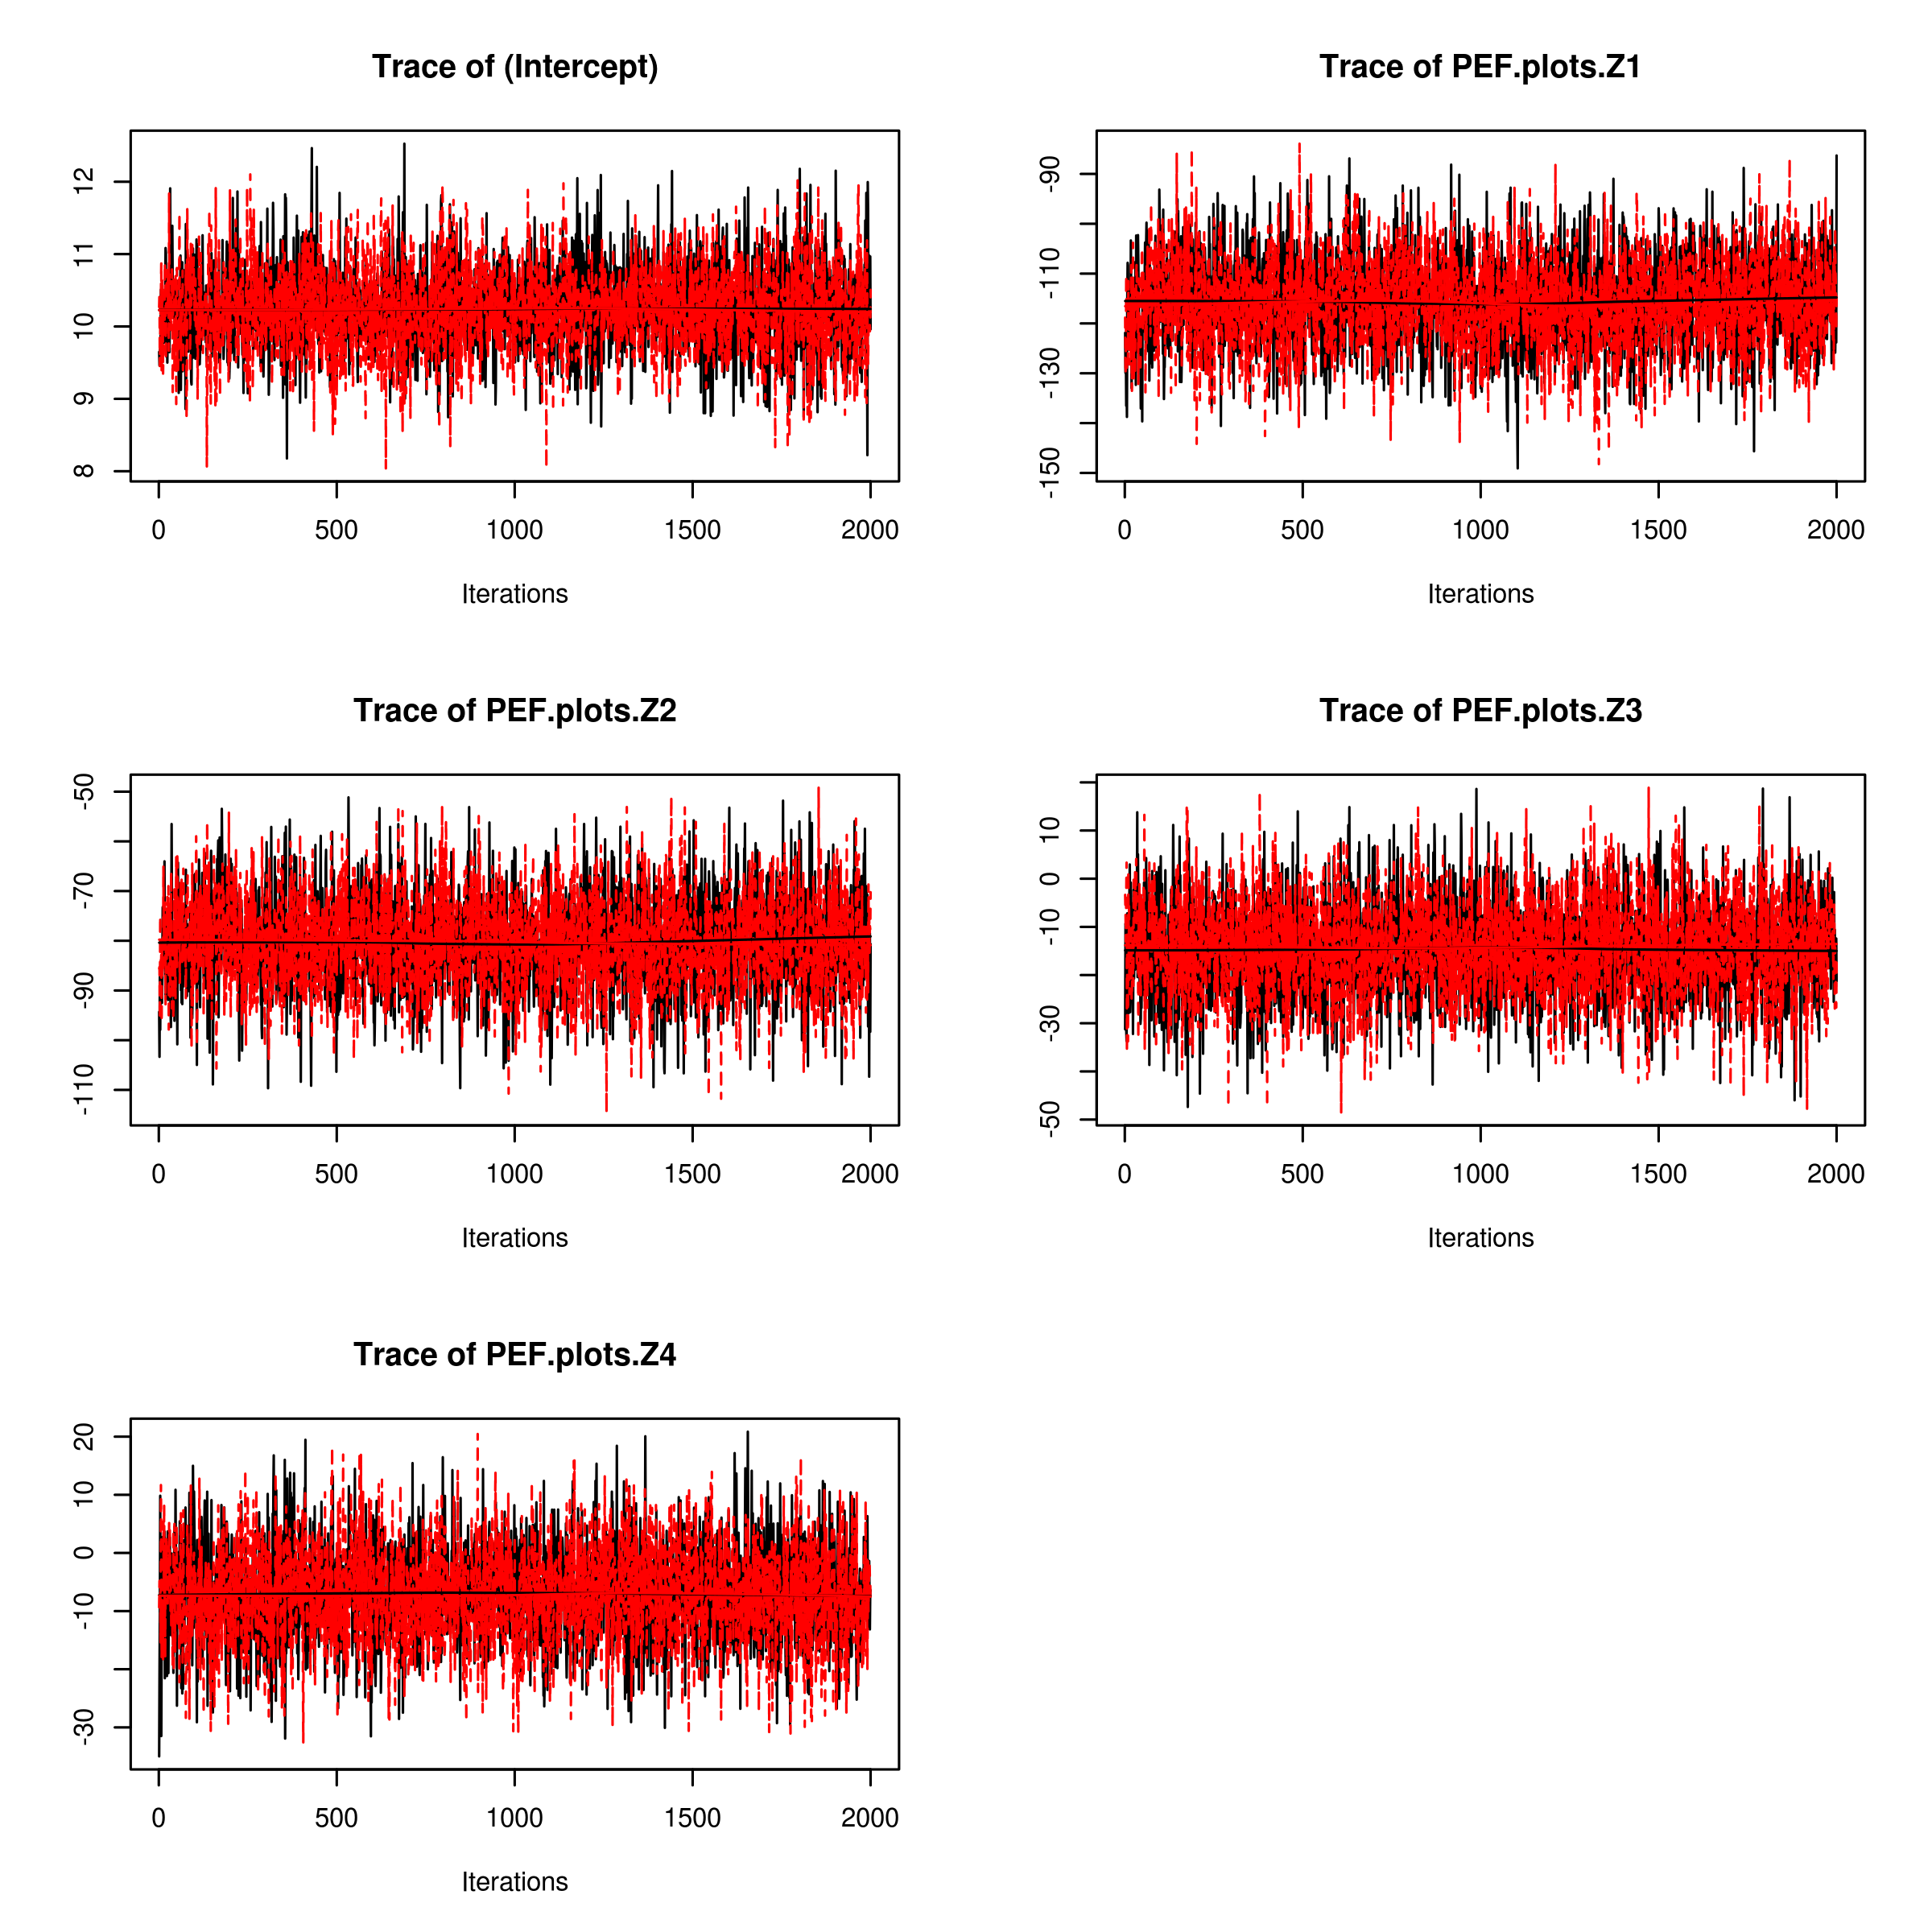
\includegraphics[width=12cm]{figures/fig-betaSamples}
\end{center}
\caption{MCMC trace plots of regression coefficients.}
\label{fig:betaSamples}
\end{figure}

\begin{Schunk}
\begin{Sinput}
> theta.samps <- mcmc.list(m.1$p.theta.samples, m.2$p.theta.samples)
> round(summary(theta.samps)$quantiles, 3)
\end{Sinput}
\begin{Soutput}
          2.5%   25%   50%   75% 97.5%
sigma.sq 2.086 2.775 3.284 3.808 5.052
tau.sq   0.551 0.780 0.926 1.082 1.389
phi      0.002 0.002 0.002 0.003 0.004
\end{Soutput}
\end{Schunk}

\begin{Schunk}
\begin{Sinput}
> burn.in <- 0.75 * n.samples
> m.1 <- spRecover(m.1, start = burn.in, thin = 10)
\end{Sinput}
\begin{Soutput}
-------------------------------------------------
		Recovering w
-------------------------------------------------
\end{Soutput}
\begin{Sinput}
> m.2 <- spRecover(m.2, start = burn.in, thin = 10)
\end{Sinput}
\begin{Soutput}
-------------------------------------------------
		Recovering w
-------------------------------------------------
\end{Soutput}
\begin{Sinput}
> m.1.w <- m.1$p.w.recover.samples
> m.2.w <- m.2$p.w.recover.samples
> w.samps <- cbind(m.1.w, m.2.w)
> w.summary <- apply(w.samps, 1, function(x) {
+     quantile(x, prob = c(0.025, 0.5, 0.975))
+ })
> w.surf <- mba.surf(cbind(coords, w.summary[2, ]), no.X = 200, no.Y = 200)$xyz.est
> z.lim <- range(w.surf[["z"]], resid.surf[["z"]], na.rm = TRUE)
> par(mfrow = c(1, 2))
> image.plot(resid.surf, zlim = z.lim, xaxs = "r", yaxs = "r", main = "Non-spatial model residuals", 
+     xlab = "Easting (m)", ylab = "Northing (m)")
> plot(PEF.shp, add = TRUE, usePolypath = FALSE)
> points(coords)
> image.plot(w.surf, zlim = z.lim, xaxs = "r", yaxs = "r", main = "Spatial random effects", 
+     xlab = "Easting (m)", ylab = "Northing (m)")
> plot(PEF.shp, add = TRUE, usePolypath = FALSE)
> points(coords)
> points(m.1$knot.coords, pch = 19, cex = 0.5)
\end{Sinput}
\end{Schunk}

\begin{figure}
\begin{center}
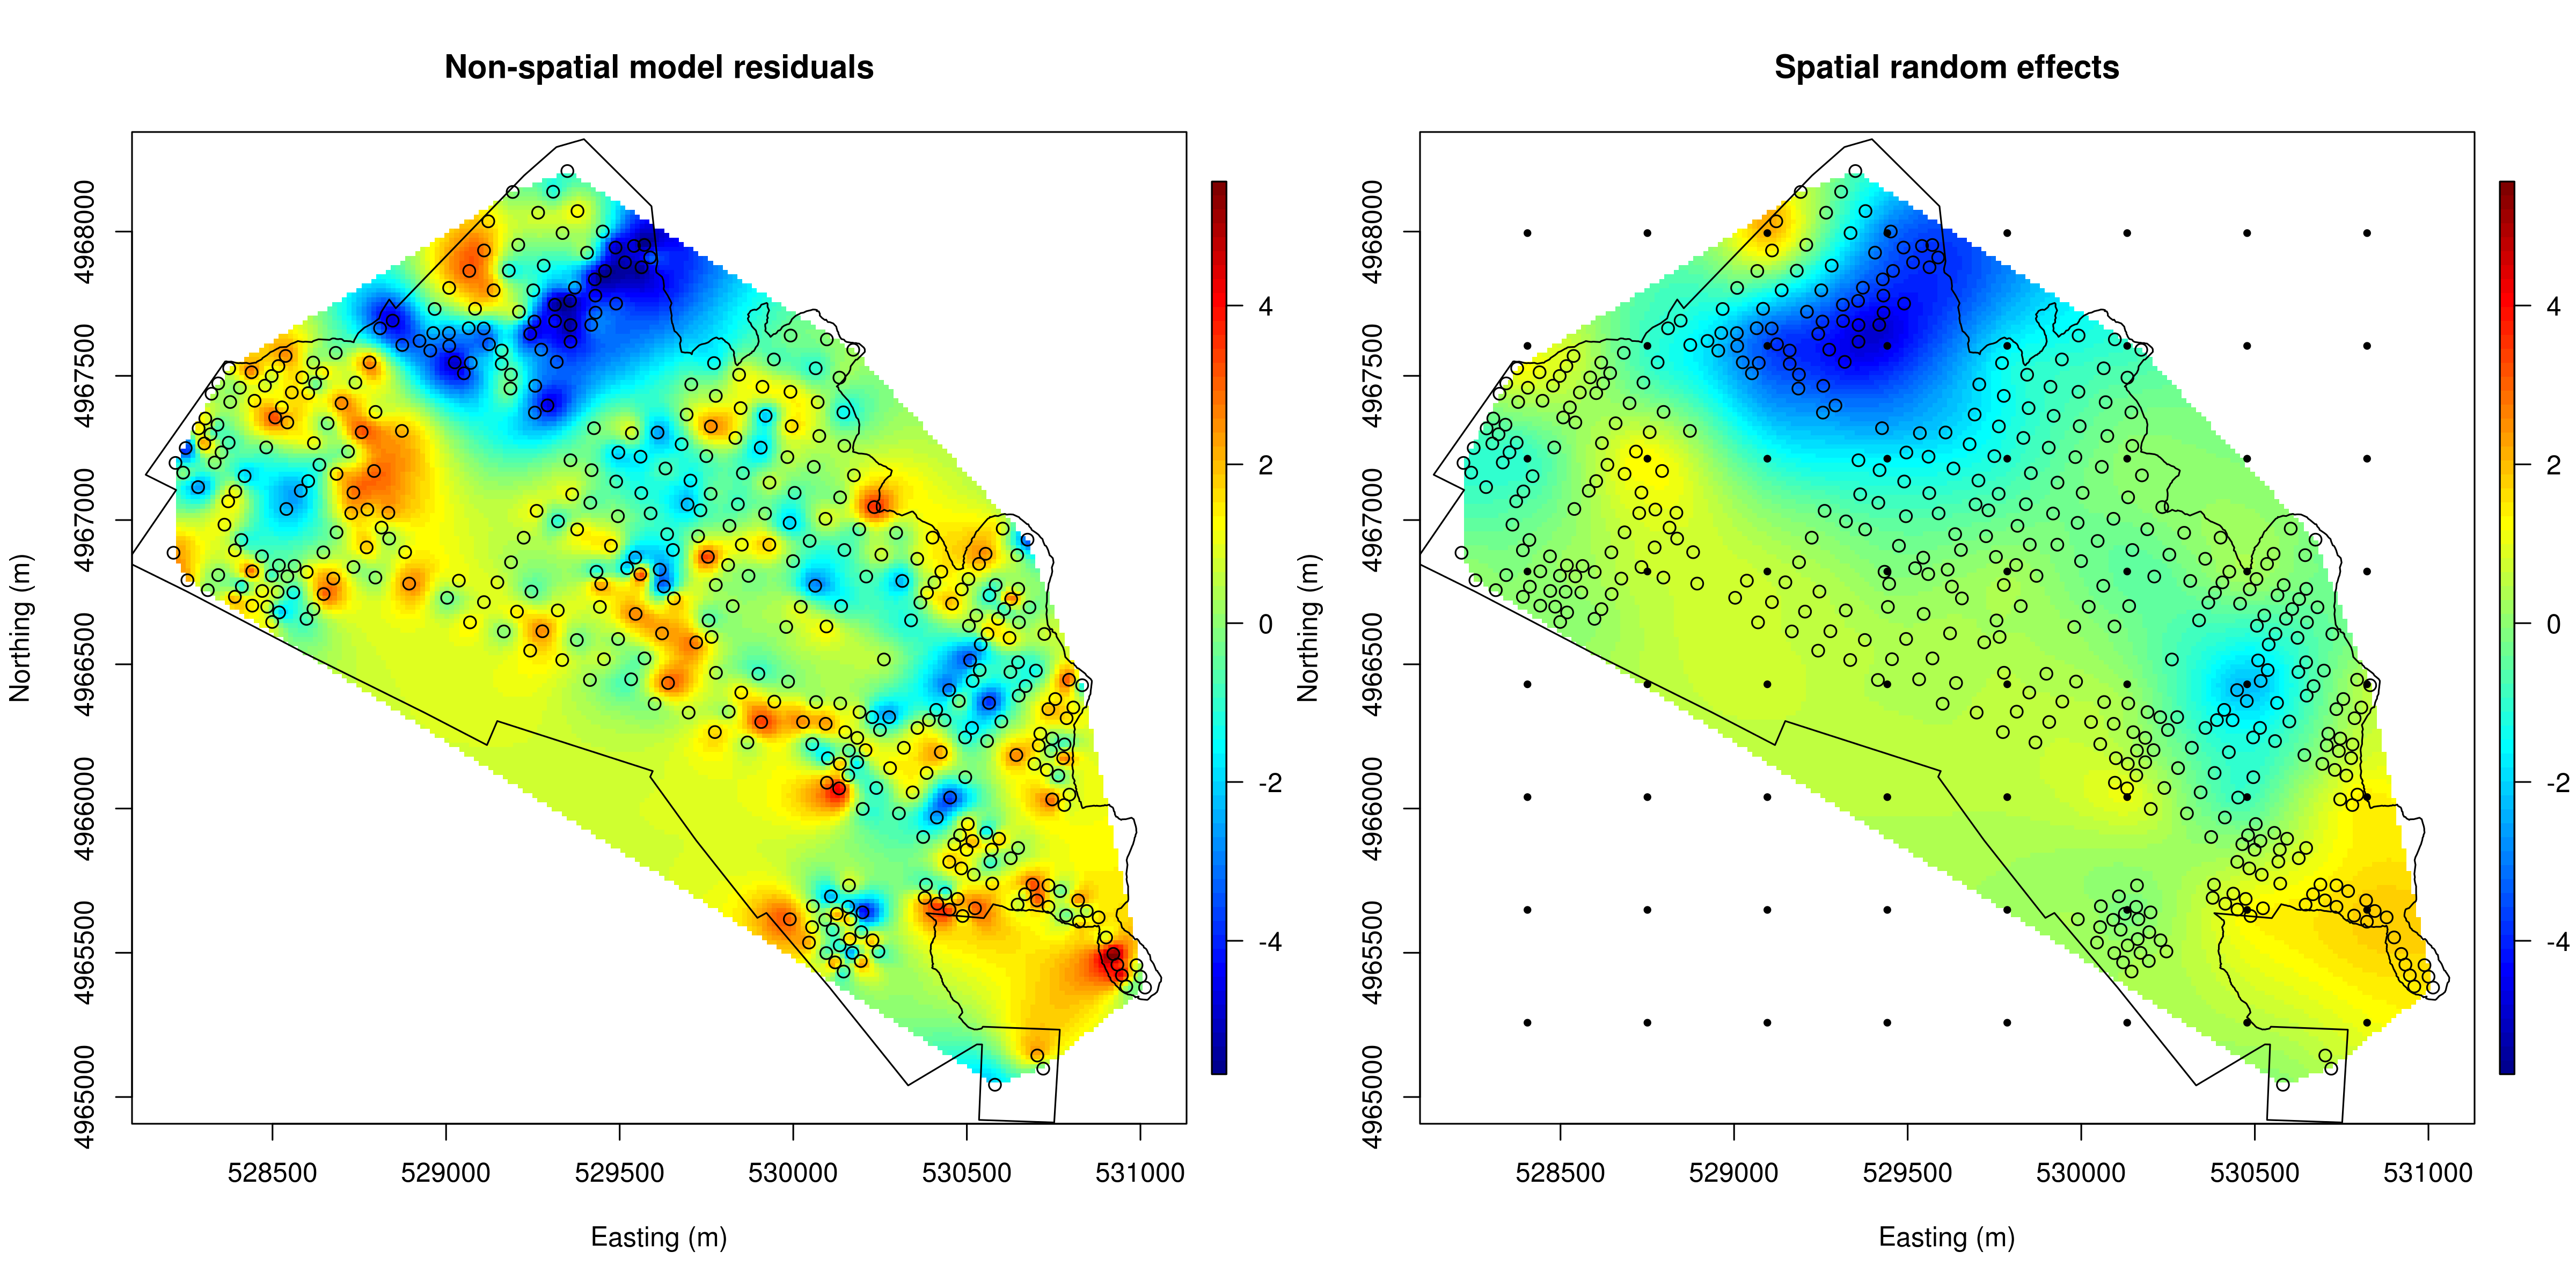
\includegraphics[width=16cm]{figures/fig-wSamples}
\end{center}
\caption{Interpolation of square-root metric tons of biomass non-spatial model residuals (left) and median of the spatial random effects posterior distributions (right).}
\label{fig:MBAResids}
\end{figure}

\subsection{Model selection}
To compare several alternative models with varying degrees of richness, we might use the GP criterion (Gelfand and Ghosh, 1998), the Deviance Information Criterion (DIC) (Spiegelhalter et al., 2002), and/or GRS scoring rule ( Gneiting and Raftery, 2007).	Using these criteria we compare the non-spatial and spatial models. Lower values of GP and DIC lower indicate improved fit, whereas for GRS higher is better. As shown below, all criteria support the addition of spatial random effects. 

\begin{Schunk}
\begin{Sinput}
> m <- lm(bio ~ PEF.plots.Z)
> m.4 <- bayesLMRef(m, n.samples)
> spDiag(m.4, start = burn.in)
\end{Sinput}
\begin{Soutput}
-------------------------------------------------
		Calculating scores
-------------------------------------------------
$DIC
                  value
bar.D       1046.666385
D.bar.Omega 1040.421252
pD             6.245133
DIC         1052.911518

$GP
     value
G 1672.101
P 1705.799
D 3377.900

$GRS
[1] -914.812
\end{Soutput}
\begin{Sinput}
> spDiag(m.1, start = burn.in)
\end{Sinput}
\begin{Soutput}
-------------------------------------------------
		Calculating scores
-------------------------------------------------
$DIC
                value
bar.D       765.32646
D.bar.Omega 732.48409
pD           32.84237
DIC         798.16884

$GP
      value
G  854.2285
P 1042.8356
D 1897.0642

$GRS
[1] -522.8122
\end{Soutput}
\end{Schunk}

\clearpage

\section{References}

\begin{description}

\item Banerjee, S., Carlin, B.P., and Gelfand, A.E. (2004). \emph{Hierarchical Modeling and Analysis for Spatial Data}, Boca Raton, FL: Chapman and Hall/CRC Press.

\item Bivand, R.B., Pebesma, E.J.,  and G\'{o}mez-Rubio, V. (2008). \emph{Applied Spatial Data Analysis with R}, UseR! Series, Springer.

\item Diggle, P.J. and Riberio, P.J. (2007). \emph{Model-based Geostatistics}, Series in Statistics, Springer.

\item Gelfand A.E. and Ghosh, S.K. (1998). Model choice: a minimum posterior predictive loss approach. \emph{Biomerika}. 85:1-11.   
  
\item Gelman, A., Carlin, J.B., Stern, H.S., and Rubin, D.B. (2004). \emph{Bayesian Data Analysis}. Second Edition. Boca Raton, FL: Chapman and Hall/CRC Press.
  
\item Gneiting, T. and Raftery, A.E. (2007). Strictly proper scoring rules, prediction, and estimation. \emph{Journal of the American Statistical Association}. 102:359-378. 
  
\item Spiegelhalter, D.J., Best, N.G., Carlin, B.P., and van der Linde, A. (2002). Bayesian measures of model complexity and fit (with discussion). \emph{Journal of the Royal Statistical Society, Series B} \textbf{64}, 583--639.
  
\end{description}
 
\end{document}
